\documentclass[12pt, a4paper]{article}

%%%%% Packages

\usepackage{verbatim}
\usepackage[width=18.8cm, left=1.1cm, height=25.9cm, top=1.7cm]{geometry}
\usepackage{amsmath,graphicx}
\usepackage{amssymb, amsthm}
\usepackage{color, enumitem}
\usepackage{arcs} %\overarc{...} arc of circle
\usepackage{pifont}
\usepackage{soul}
\usepackage{wrapfig}
\usepackage{fancybox}
\usepackage{harpoon}
\usepackage{pgfplots}
\usepackage{tikz}
\usetikzlibrary{positioning}
\usetikzlibrary{shapes.multipart}
\usepackage{fancyhdr}
\pagestyle{fancy}
\renewcommand{\familydefault}{\rmdefault}
\usepackage{multicol}
\setlength{\parindent}{0cm}
\usepackage{fontspec} %加這個就可以設定字體
\usepackage{fourier}
\usepackage{cleveref}
\usepackage[most]{tcolorbox}
\usepackage{lipsum}
\usepackage[framemethod=TikZ]{mdframed}
\usepackage[hidelinks,hypertexnames=false]{hyperref}
\usepackage{xparse}
\usepackage{titlesec}
\usepackage{mathtools}


%%%%% Header and Footer

\renewcommand{\headrulewidth}{0pt}
\rhead{}

\cfoot{P. \thepage}

%%%%% Sbullet

\newcommand\sbullet[1][1]{\mathbin{\vcenter{\hbox{\scalebox{#1}{$\bullet$}}}}}


%%%%% Section Style

\titleformat{\section}
{\bf\LARGE}{\thesection.}{0.3em}{}


%%%%% MathsChris

\renewcommand{\MathsChris}{MathsChris\null}


%%%%% Recurring Decimals


\ExplSyntaxOn

%% Dots on the first and last digit
\NewDocumentCommand{\periodfl}{m}
{
  \repdec_initial_final_dots:n { #1 }
}

\seq_new:N \l__repdec_digits_seq
\tl_new:N \l__repdec_first_tl
\tl_new:N \l__repdec_last_tl

\cs_new_protected:Npn \repdec_initial_final_dots:n #1
{
  \seq_set_split:Nnn \l__repdec_digits_seq {} { #1 }
  \seq_pop_left:NN \l__repdec_digits_seq \l__repdec_first_tl
  \seq_pop_right:NN \l__repdec_digits_seq \l__repdec_last_tl
  \quark_if_no_value:VF \l__repdec_first_tl { \dot{\l__repdec_first_tl} }
  \seq_use:Nnnn \l__repdec_digits_seq {}{}{}
  \quark_if_no_value:VF \l__repdec_last_tl { \dot{\l__repdec_last_tl} }
}
\cs_generate_variant:Nn \quark_if_no_value:nF { V }

%% Dots on all digits
\NewDocumentCommand{\periodalldots}{m}
{
  \repdec_initial_all_dots:n { #1 }
}

\cs_new_protected:Npn \repdec_initial_all_dots:n #1
{
  \tl_map_inline:nn { #1 } { \dot{##1} }
}

%% Bar over period
\NewDocumentCommand{\periodbar}{m}
{
  \overline{ #1 }
}

%% Parentheses around period
\NewDocumentCommand{\periodparens}{m}
{
  (#1)
}

%% Dot on unique digit, bar on several digits
\NewDocumentCommand{\periodmixed}{m}
{
  \repdec_mixed:n { #1 }
}
\cs_new_protected:Npn \repdec_mixed:n #1
{
  \int_case:nnn { \tl_count:n { #1 } }
  {
    { 0 } { }
      { 1 } { \dot{#1} }
  }
  {
    \overline{#1}
  }
}

\ExplSyntaxOff

%%%%%






%%%%% enumitem setting
\setlistdepth{9}
\newlist{enumprob}{enumerate}{9}
\setenumerate[enumprob]{leftmargin=8mm,rightmargin=0pt,label=\arabic*.,labelwidth=8mm, itemsep=6mm, topsep=0mm, labelsep=2mm, labelindent=0pt, align=left, partopsep=5mm}
\setlist[enumprob,1]{label=\arabic*.,widest=999,itemindent=0pt,labelsep=2mm,labelwidth=6mm}
\setlist[enumprob,2]{label=(\alph*)}
\setlist[enumprob,3]{label=(\roman*)}
\setlist[enumprob,4]{label=(\arabic*)}
\setlist[enumprob,5]{label=(\arabic*)}
\setlist[enumprob,6]{label=(\arabic*)}
\setlist[enumprob,7]{label=(\arabic*)}
\setlist[enumprob,8]{label=(\arabic*)}
\setlist[enumprob,9]{label=(\arabic*)}



\setlistdepth{9}
\newlist{enumx}{enumerate}{9}
\setenumerate[enumx]{leftmargin=0.8cm,rightmargin=0pt,label=\arabic*.,labelwidth=6mm, itemsep=3pt, topsep=3mm, labelsep=2mm, labelindent=0pt, align=left, partopsep=0mm}
\setlist[enumx,1]{label=\arabic*.}
\setlist[enumx,2]{label=(\alph*),itemsep=0pt,topsep=0pt}
\setlist[enumx,3]{label=(\roman*)}
\setlist[enumx,4]{label=(\arabic*)}
\setlist[enumx,5]{label=(\arabic*)}
\setlist[enumx,6]{label=(\arabic*)}
\setlist[enumx,7]{label=(\arabic*)}
\setlist[enumx,8]{label=(\arabic*)}
\setlist[enumx,9]{label=(\arabic*)}


\setlistdepth{9}
\newlist{thinkitem}{enumerate}{9}
\setenumerate[thinkitem]{leftmargin=1.2em,rightmargin=0pt,label=\textcolor{green!80!black}{\sbullet[1.5]},itemsep=0pt,topsep=3pt}

\newlist{itemlist}{enumerate}{9}
\setenumerate[itemlist]{leftmargin=1.2em,rightmargin=0pt,label={\sbullet[1.5]},itemsep=0pt,topsep=3pt}

\setlistdepth{9}
\newlist{planitem}{enumerate}{9}
\setenumerate[planitem]{leftmargin=*,rightmargin=0pt,label=\arabic*.,itemsep=0pt,topsep=3pt,widest=99}
\setlist[planitem,1]{label=\arabic*.}
\setlist[planitem,2]{label=(\alph*)}
\setlist[planitem,3]{label=(\roman*)}
\setlist[planitem,4]{label=(\arabic*)}
\setlist[planitem,5]{label=(\arabic*)}
\setlist[planitem,6]{label=(\arabic*)}
\setlist[planitem,7]{label=(\arabic*)}
\setlist[planitem,8]{label=(\arabic*)}
\setlist[planitem,9]{label=(\arabic*)}

\newlist{steps}{enumerate}{9}
\setenumerate[steps]{leftmargin=*,rightmargin=0pt,label=Step~\arabic*.,itemsep=0pt,topsep=3pt,widest=99}
\setlist[steps,1]{label=Step \arabic*.}
\setlist[steps,2]{label=(\alph*)}
\setlist[steps,3]{label=(\roman*)}
\setlist[steps,4]{label=(\arabic*)}
\setlist[steps,5]{label=(\arabic*)}
\setlist[steps,6]{label=(\arabic*)}
\setlist[steps,7]{label=(\arabic*)}
\setlist[steps,8]{label=(\arabic*)}
\setlist[steps,9]{label=(\arabic*)}

\newlist{writesteps}{enumerate}{9}
\setenumerate[writesteps]{leftmargin=*,rightmargin=0pt,label={\small \tt \textcolor{blue}{\arabic*.}},itemsep=0pt,topsep=3pt,widest=99}
\setlist[writesteps,1]{label={\small \tt \textcolor{blue}{\arabic*.}}}
\setlist[writesteps,2]{label={\small \tt \textcolor{blue}{(\alph*)}}}
\setlist[writesteps,3]{label=(\roman*)}
\setlist[writesteps,4]{label=(\arabic*)}
\setlist[writesteps,5]{label=(\arabic*)}
\setlist[writesteps,6]{label=(\arabic*)}
\setlist[writesteps,7]{label=(\arabic*)}
\setlist[writesteps,8]{label=(\arabic*)}
\setlist[writesteps,9]{label=(\arabic*)}

\newcommand{\planstep}[1]{\ensuremath{\text{\small \tt \textcolor{blue}{[#1]}}}}




%%%%% Fonts Setting
\setmainfont{Times New Roman}
\usepackage{xeCJK}  %讓中英文字體分開設置
\setCJKmainfont{新細明體} %設定中文為系統上的字型,而英文不去更動,使用原TeX字%型
\XeTeXlinebreaklocale "zh"   %這兩行一定要加,中文才能自動換行
\XeTeXlinebreakskip = 0pt plus 1pt %這兩行一定要加,中文才能自動換行

%%%%% User Defined Functions
\newcommand{\abs}[1]{\left|#1\right|}
\newcommand{\dps}{\displaystyle}
\newcommand{\parallelsum}{\mathbin{\!/\mkern-5mu/\!}}
\renewcommand{\overarc}[1]{\widearc{#1}}
\newcommand{\any}{\forall\, }
\newcommand{\degree}{\ensuremath{^{\circ}}}
\renewcommand{\d}{\mbox{d}}

\newcommand{\NF}{
  \begin{tikzpicture}
    \node[inner sep=0.1cm, preaction={fill=black,fill opacity=0.15},rounded corners=0.1ex,font=\fontsize{7pt}{17pt}\selectfont] (c) {\textbf{NF}}
  \end{tikzpicture}
}

%%% Vectors
\renewcommand{\i}{\mathbf{i}}
\renewcommand{\j}{\mathbf{j}}
\renewcommand{\k}{\mathbf{k}}
\renewcommand{\vec}[1]{\overrightharp{#1}}

%%%%% Marking Style
\renewcommand{\marks}[1]{\hfill\null\hfill (#1~marks)}
\newcommand{\onemark}{\hfill\null\hfill (1~mark)}

%%%%% Graphics

\newcommand{\graphics}[1]{\par
  \begin{center}
    \includegraphics{#1}
  \end{center}
}

\graphicspath{{D:/DSEbyTopic/Graphics/}}

\newcommand{\mcgraphics}[2]{
  \null\par
  \vspace{-3mm}
  \begin{minipage}[t]{0.45\textwidth}

    #2

  \end{minipage}
  \begin{minipage}[t]{0.5\textwidth}
    \null\par
    \vspace{-0.02\textwidth}

    \begin{flushright}
      \includegraphics{#1}
    \end{flushright}
  \end{minipage}
  \vspace{0.01\textwidth}
}


%%%%% Environments

\newenvironment{absolutelynopagebreak}
{\nobreak\vfil\penalty0\vfilneg
  \vtop\bgroup}
{\par\xdef\tpd{\the\prevdepth}\egroup
  \prevdepth=\tpd}

\newcommand{\greybox}[1]{
  \begin{tikzpicture}
    \node[inner sep=0.3cm, preaction={fill=black,fill opacity=0.15},rounded corners=1ex,font=\fontsize{24pt}{24pt}\selectfont] (c) {#1}
  \end{tikzpicture}
}

\SetLabelAlign{parright}{\parbox[t]{\labelwidth}{\raggedleft‌​#1}}


%%%%% get and put

\newcommand{\sectiontitle}[3]{\input{"D:/DSEbyTopic/SectionTitle/Title_#1_#2_#3.tex"}}


\newcommand{\problem}[2][]{
  \begin{minipage}[t]{(\textwidth-1cm)}
    \input{"D:/DSEbyTopic/Problems/#2.tex"}%
    \ifstrempty{#1}%
    {
    }%
    {\linebreak\null\hfill[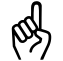
\includegraphics{uppointing}#2]
    }%
  \end{minipage}
}



\newcommand{\problemans}[1]{
  \begin{minipage}[t]{(\textwidth-1cm)}
    \input{"D:/DSEbyTopic/Problems/#1-ans.tex"}
  \end{minipage}
}


%%%%% Graphics


\newcommand{\starr}{
\includegraphics{star}}

\graphicspath{{D:/DSEbyTopic/Graphics/}}

\newcommand{\mcgraphics}[2]{
  \par
  \vspace{0.0001\textwidth}
  \begin{minipage}[t]{0.33\textwidth}

    #2

  \end{minipage}
  \begin{minipage}[t]{0.65\textwidth}
    \null\par
    \vspace{-0.12\textwidth}

    \begin{flushright}
      \includegraphics{#1}
    \end{flushright}
  \end{minipage}
  \vspace{0.01\textwidth}
}



%%%%% environment commands


%%%%% TC environment

\newcounter{tccounter}
\setcounter{tccounter}{0}
\renewcommand{\thetccount}{\arabic{tccounter}}
\newenvironment{theorem}[2][]{%
  \refstepcounter{tccounter}%
  \ifstrempty{#1}%
  {\mdfsetup{%
      frametitle={%
          \tikz[baseline=(current bounding box.east),outer sep=0pt]
          \node[anchor=east,rectangle,fill=blue!20]
          {\strut Theorem~\thetccount};}}
  }%
  {\mdfsetup{%
      frametitle={%
          \tikz[baseline=(current bounding box.east),outer sep=0pt]
          \node[anchor=east,rectangle,fill=blue!20]
          {\strut Theorem~\thetccount~(#1)~};}}%
  }%
  \mdfsetup{innertopmargin=4pt,innerbottommargin=10pt,linecolor=blue!20,%
    linewidth=2pt,topline=true,%
    frametitleaboveskip=\dimexpr-\ht\strutbox\relax
  }
  \begin{mdframed}[]\relax%
    \label{#2}}{\end{mdframed}}

\newenvironment{concept}[2][]{%
  \refstepcounter{tccounter}%
  \ifstrempty{#1}%
  {\mdfsetup{%
      frametitle={%
          \tikz[baseline=(current bounding box.east),outer sep=0pt]
          \node[anchor=east,rectangle,fill=blue!20]
          {\strut Concept~\thetccount};}}
  }%
  {\mdfsetup{%
      frametitle={%
          \tikz[baseline=(current bounding box.east),outer sep=0pt]
          \node[anchor=east,rectangle,fill=blue!20]
          {\strut Concept~\thetccount~(#1)~};}}%
  }%
  \mdfsetup{innertopmargin=4pt,innerbottommargin=10pt,linecolor=blue!20,%
    linewidth=2pt,topline=true,%
    frametitleaboveskip=\dimexpr-\ht\strutbox\relax
  }
  \begin{mdframed}[]\relax%
    \label{#2}}{\end{mdframed}}

\newenvironment{formula}[2][]{%
  \refstepcounter{tccounter}%
  \ifstrempty{#1}%
  {\mdfsetup{%
      frametitle={%
          \tikz[baseline=(current bounding box.east),outer sep=0pt]
          \node[anchor=east,rectangle,fill=blue!20]
          {\strut Formula~\thetccount};}}
  }%
  {\mdfsetup{%
      frametitle={%
          \tikz[baseline=(current bounding box.east),outer sep=0pt]
          \node[anchor=east,rectangle,fill=blue!20]
          {\strut Formula~\thetccount~(#1)~};}}%
  }%
  \mdfsetup{innertopmargin=4pt,innerbottommargin=10pt,linecolor=blue!20,%
    linewidth=2pt,topline=true,%
    frametitleaboveskip=\dimexpr-\ht\strutbox\relax
  }
  \begin{mdframed}[]\relax%
    \label{#2}}{\end{mdframed}}


\newenvironment{presentation}[2][]{%
  \refstepcounter{tccounter}%
  \ifstrempty{#1}%
  {\mdfsetup{%
      frametitle={%
          \tikz[baseline=(current bounding box.east),outer sep=0pt]
          \node[anchor=east,rectangle,fill=blue!20]
          {\strut Presentation~\thetccount};}}
  }%
  {\mdfsetup{%
      frametitle={%
          \tikz[baseline=(current bounding box.east),outer sep=0pt]
          \node[anchor=east,rectangle,fill=blue!20]
          {\strut Presentation~\thetccount~(#1)~};}}%
  }%
  \mdfsetup{innertopmargin=4pt,innerbottommargin=10pt,linecolor=blue!20,%
    linewidth=2pt,topline=true,%
    frametitleaboveskip=\dimexpr-\ht\strutbox\relax
  }
  \begin{mdframed}[]\relax%
    \label{#2}}{\end{mdframed}}


%%%%% LP environment

\newcounter{lpcounter}
\setcounter{lpcounter}{0}
\renewcommand{\thelpcount}{\arabic{lpcounter}}

\newenvironment{skill}[2][]{%
  \refstepcounter{lpcounter}%
  \ifstrempty{#1}%
  {\mdfsetup{%
      frametitle={%
          \tikz[baseline=(current bounding box.east),outer sep=0pt]
          \node[anchor=east,rectangle,fill=red!20]
          {\strut Skill~\thelpcount};}}
  }%
  {\mdfsetup{%
      frametitle={%
          \tikz[baseline=(current bounding box.east),outer sep=0pt]
          \node[anchor=east,rectangle,fill=red!20]
          {\strut Skill~\thelpcount~(#1)~};}}%
  }%
  \mdfsetup{innertopmargin=4pt,innerbottommargin=10pt,linecolor=red!20,%
    linewidth=2pt,topline=true,%
    frametitleaboveskip=\dimexpr-\ht\strutbox\relax
  }
  \begin{mdframed}[]\relax%
    \label{#2}}{\end{mdframed}}


\newenvironment{trick}[2][]{%
  \refstepcounter{lpcounter}%
  \ifstrempty{#1}%
  {\mdfsetup{%
      frametitle={%
          \tikz[baseline=(current bounding box.east),outer sep=0pt]
          \node[anchor=east,rectangle,fill=red!20]
          {\strut Trick~\thelpcount};}}
  }%
  {\mdfsetup{%
      frametitle={%
          \tikz[baseline=(current bounding box.east),outer sep=0pt]
          \node[anchor=east,rectangle,fill=red!20]
          {\strut Trick~\thelpcount~(#1)~};}}%
  }%
  \mdfsetup{innertopmargin=4pt,innerbottommargin=10pt,linecolor=red!20,%
    linewidth=2pt,topline=true,%
    frametitleaboveskip=\dimexpr-\ht\strutbox\relax
  }
  \begin{mdframed}[]\relax%
    \label{#2}}{\end{mdframed}}


\newenvironment{fact}[2][]{%
  \refstepcounter{lpcounter}%
  \ifstrempty{#1}%
  {\mdfsetup{%
      frametitle={%
          \tikz[baseline=(current bounding box.east),outer sep=0pt]
          \node[anchor=east,rectangle,fill=red!20]
          {\strut Fact~\thelpcount};}}
  }%
  {\mdfsetup{%
      frametitle={%
          \tikz[baseline=(current bounding box.east),outer sep=0pt]
          \node[anchor=east,rectangle,fill=red!20]
          {\strut Fact~\thelpcount~(#1)~};}}%
  }%
  \mdfsetup{innertopmargin=4pt,innerbottommargin=10pt,linecolor=red!20,%
    linewidth=2pt,topline=true,%
    frametitleaboveskip=\dimexpr-\ht\strutbox\relax
  }
  \begin{mdframed}[]\relax%
    \label{#2}}{\end{mdframed}}


\newenvironment{skillgroup}[2][]{%
  \refstepcounter{lpcounter}%
  \ifstrempty{#1}%
  {\mdfsetup{%
      frametitle={%
          \tikz[baseline=(current bounding box.east),outer sep=0pt]
          \node[anchor=east,rectangle,fill=red!20]
          {\strut Skill Group~\thelpcount};}}
  }%
  {\mdfsetup{%
      frametitle={%
          \tikz[baseline=(current bounding box.east),outer sep=0pt]
          \node[anchor=east,rectangle,fill=red!20]
          {\strut Skill Group~\thelpcount~(#1)~};}}%
  }%
  \mdfsetup{innertopmargin=4pt,innerbottommargin=10pt,linecolor=red!20,%
    linewidth=2pt,topline=true,%
    frametitleaboveskip=\dimexpr-\ht\strutbox\relax
  }
  \begin{mdframed}[]\relax%
    \label{#2}}{\end{mdframed}}


\newenvironment{trickgroup}[2][]{%
  \refstepcounter{lpcounter}%
  \ifstrempty{#1}%
  {\mdfsetup{%
      frametitle={%
          \tikz[baseline=(current bounding box.east),outer sep=0pt]
          \node[anchor=east,rectangle,fill=red!20]
          {\strut Trick Group~\thelpcount};}}
  }%
  {\mdfsetup{%
      frametitle={%
          \tikz[baseline=(current bounding box.east),outer sep=0pt]
          \node[anchor=east,rectangle,fill=red!20]
          {\strut Trick Group~\thelpcount~(#1)~};}}%
  }%
  \mdfsetup{innertopmargin=4pt,innerbottommargin=10pt,linecolor=red!20,%
    linewidth=2pt,topline=true,%
    frametitleaboveskip=\dimexpr-\ht\strutbox\relax
  }
  \begin{mdframed}[]\relax%
    \label{#2}}{\end{mdframed}}


\newenvironment{factgroup}[2][]{%
  \refstepcounter{lpcounter}%
  \ifstrempty{#1}%
  {\mdfsetup{%
      frametitle={%
          \tikz[baseline=(current bounding box.east),outer sep=0pt]
          \node[anchor=east,rectangle,fill=red!20]
          {\strut Fact Group~\thelpcount};}}
  }%
  {\mdfsetup{%
      frametitle={%
          \tikz[baseline=(current bounding box.east),outer sep=0pt]
          \node[anchor=east,rectangle,fill=red!20]
          {\strut Fact Group~\thelpcount~(#1)~};}}%
  }%
  \mdfsetup{innertopmargin=4pt,innerbottommargin=10pt,linecolor=red!20,%
    linewidth=2pt,topline=true,%
    frametitleaboveskip=\dimexpr-\ht\strutbox\relax
  }
  \begin{mdframed}[]\relax%
    \label{#2}}{\end{mdframed}}

\newenvironment{pattern}[2][]{%
  \refstepcounter{lpcounter}%
  \ifstrempty{#1}%
  {\mdfsetup{%
      frametitle={%
          \tikz[baseline=(current bounding box.east),outer sep=0pt]
          \node[anchor=east,rectangle,fill=red!20]
          {\strut Pattern~\thelpcount};}}
  }%
  {\mdfsetup{%
      frametitle={%
          \tikz[baseline=(current bounding box.east),outer sep=0pt]
          \node[anchor=east,rectangle,fill=red!20]
          {\strut Pattern~\thelpcount~(#1)~};}}%
  }%
  \mdfsetup{innertopmargin=4pt,innerbottommargin=10pt,linecolor=red!20,%
    linewidth=2pt,topline=true,%
    frametitleaboveskip=\dimexpr-\ht\strutbox\relax
  }
  \begin{mdframed}[]\relax%
    \label{#2}}{\end{mdframed}}


\newcounter{illucounter}[lpcounter]
\setcounter{illucounter}{0}
\renewcommand{\theillucounter}{\thelpcounter.\arabic{illucounter}}

\newenvironment{illustration}[2][]{%
  \refstepcounter{illucounter}%
  \ifstrempty{#1}%
  {\mdfsetup{%
      frametitle={%
          \tikz[baseline=(current bounding box.east),outer sep=0pt]
          \node[anchor=east,rectangle,fill=red!10]
          {\strut Illustration~\theillucounter};}}
  }%
  {\mdfsetup{%
      frametitle={%
          \tikz[baseline=(current bounding box.east),outer sep=0pt]
          \node[anchor=east,rectangle,fill=red!10]
          {\strut Illustration~\theillucounter~(#1)~};}}%
  }%
  \mdfsetup{innertopmargin=4pt,innerbottommargin=10pt,linecolor=red!10,%
    linewidth=2pt,topline=true,%
    frametitleaboveskip=\dimexpr-\ht\strutbox\relax
  }
  \begin{mdframed}[]\relax%
    \label{#2}}{\end{mdframed}}

\newenvironment{tiy}[2][]{%
  \refstepcounter{illucounter}%
  \ifstrempty{#1}%
  {\mdfsetup{%
      frametitle={%
          \tikz[baseline=(current bounding box.east),outer sep=0pt]
          \node[anchor=east,rectangle,fill=red!20]
          {\strut Try it Yourself~\theillucounter};}}
  }%
  {\mdfsetup{%
      frametitle={%
          \tikz[baseline=(current bounding box.east),outer sep=0pt]
          \node[anchor=east,rectangle,fill=red!20]
          {\strut Try it Yourself~\theillucounter~(#1)~};}}%
  }%
  \mdfsetup{innertopmargin=4pt,innerbottommargin=10pt,linecolor=red!20,%
    linewidth=2pt,topline=true,%
    frametitleaboveskip=\dimexpr-\ht\strutbox\relax
  }
  \begin{mdframed}[]\relax%
    \label{#2}}{\end{mdframed}}



%%%%% Eg Environments

\newcounter{egcounter}
\setcounter{egcounter}{0}
\renewcommand{\theegcount}{\arabic{egcounter}}
\newenvironment{example}[2][]{%
  \begin{absolutelynopagebreak}
    \refstepcounter{egcounter}%
    \ifstrempty{#1}%
    {\mdfsetup{%
        frametitle={%
            \tikz[baseline=(current bounding box.east),outer sep=0pt]
            \node[anchor=east,rectangle,fill=green!40]
            {\strut Example~\theegcount};}}
    }%
    {\mdfsetup{%
        frametitle={%
            \tikz[baseline=(current bounding box.east),outer sep=0pt]
            \node[anchor=east,rectangle,fill=green!40]
            {\strut Example~\theegcount~(#1)~};}}%
    }%
    \mdfsetup{innertopmargin=4pt,innerbottommargin=10pt,linecolor=green!40,%
      linewidth=2pt,topline=true,%
      frametitleaboveskip=\dimexpr-\ht\strutbox\relax,
      skipabove=0pt,skipbelow=25pt,
    }
    \begin{mdframed}[]\relax%
      \label{#2}}{\end{mdframed}\end{absolutelynopagebreak}}


\newenvironment{Question}[2][]{%
  \begin{absolutelynopagebreak}
    \refstepcounter{egcounter}%
    \ifstrempty{#1}%
    {\mdfsetup{%
        frametitle={%
            \tikz[baseline=(current bounding box.east),outer sep=0pt]
            \node[anchor=east,rectangle,fill=green!40]
            {\strut Example~\ref{#2}};}}
    }%
    {\mdfsetup{%
        frametitle={%
            \tikz[baseline=(current bounding box.east),outer sep=0pt]
            \node[anchor=east,rectangle,fill=green!40]
            {\strut Example~\ref{#2}~(#1)~};}}%
    }%
    \mdfsetup{innertopmargin=4pt,innerbottommargin=10pt,linecolor=green!40,%
      linewidth=2pt,topline=true,%
      frametitleaboveskip=\dimexpr-\ht\strutbox\relax,
      skipabove=0pt,skipbelow=25pt,
    }
    \begin{mdframed}[]\relax%
      }{\end{mdframed}\end{absolutelynopagebreak}}






\newenvironment{Read}{%
  \begin{mdframed}[%
      frametitle={
\includegraphics{Read}~Read the Question},
      apptotikzsetting={\tikzset{mdfframetitlebackground/.append style={%
              shade,left color=green!20!white, right color=white}}},
      %frametitlerule=true,
      %frametitlerulewidth=1pt,
      %frametitlerulecolor=black,
      innertopmargin=0.7em,%
      innerleftmargin=0.7em,%,
      innerrightmargin=0.7em,
      hidealllines=true,leftline=true,
      frametitlebackgroundcolor=green!20,
      linewidth=3pt,
      linecolor=green!20,
      skipabove=0pt,skipbelow=0pt,
      %fontcolor=white,%
      %backgroundcolor=green!10
    ]%
    }{%
  \end{mdframed}
}

\newcommand{\readrule}{\textcolor{green!80!black}{\hrulefill}}
\newcommand{\illustrationrule}{\textcolor{red!10}{\hrulefill}}



\newenvironment{Think}{%
  \begin{mdframed}[%
      frametitle={
\includegraphics{Think}~Thinking Process},
      apptotikzsetting={\tikzset{mdfframetitlebackground/.append style={%
              shade,left color=green!20!white, right color=white}}},
      %frametitlerule=true,
      %frametitlerulewidth=1pt,
      %frametitlerulecolor=black,
      innertopmargin=0.7em,%
      innerleftmargin=0.7em,%,
      innerrightmargin=0.7em,
      hidealllines=true,leftline=true,
      frametitlebackgroundcolor=green!20,
      linewidth=3pt,
      linecolor=green!20,
      skipabove=0pt,skipbelow=0pt,
      %fontcolor=white,%
      %backgroundcolor=green!10
    ]%
    }{%
  \end{mdframed}
}

\newenvironment{Plan}{%
  \begin{mdframed}[%
      frametitle={
\includegraphics{Plan}~Plan of Attack},
      apptotikzsetting={\tikzset{mdfframetitlebackground/.append style={%
              shade,left color=green!20!white, right color=white}}},
      %frametitlerule=true,
      %frametitlerulewidth=1pt,
      %frametitlerulecolor=black,
      innertopmargin=0.7em,%
      innerleftmargin=0.7em,%,
      innerrightmargin=0.7em,
      hidealllines=true,leftline=true,
      frametitlebackgroundcolor=green!20,
      linewidth=3pt,
      linecolor=green!20,
      skipabove=0pt,skipbelow=0pt,
      %fontcolor=white,%
      %backgroundcolor=green!10
    ]%
    }{%
  \end{mdframed}
}

\newenvironment{Remark}{%
  \begin{mdframed}[%
      frametitle={Remarks and Comments},
      apptotikzsetting={\tikzset{mdfframetitlebackground/.append style={%
              shade,left color=green!20!white, right color=white}}},
      %frametitlerule=true,
      %frametitlerulewidth=1pt,
      %frametitlerulecolor=black,
      innertopmargin=0.7em,%
      innerleftmargin=0.7em,%,
      innerrightmargin=0.7em,
      hidealllines=true,leftline=true,
      frametitlebackgroundcolor=green!20,
      linewidth=3pt,
      linecolor=green!20,
      skipabove=0pt,skipbelow=0pt,
      %fontcolor=white,%
      %backgroundcolor=green!10
    ]%
    }{%
  \end{mdframed}
}

\newenvironment{Write}{%
  \begin{mdframed}[%
      frametitle={
\includegraphics{Write}~What to Write},
      apptotikzsetting={\tikzset{mdfframetitlebackground/.append style={%
              shade,left color=green!30!white, right color=white}}},
      %frametitlerule=true,
      %frametitlerulewidth=1pt,
      %frametitlerulecolor=black,
      innertopmargin=0.7em,%
      innerleftmargin=0.7em,%,
      innerrightmargin=0.7em,
      hidealllines=true,leftline=true, bottomline=true,
      frametitlebackgroundcolor=green!30,
      linewidth=3pt,
      linecolor=green!30,
      %fontcolor=white,%
      %backgroundcolor=green!10
    ]%
    \large
    }{%
  \end{mdframed}
}






%%%%% highlight box


\newtcbox{\lbox}{enhanced,nobeforeafter,tcbox raise base,boxrule=1.3pt,top=0mm,bottom=0mm,right=0.05mm,left=0.05mm,arc=0pt,boxsep=2pt,before upper={\vphantom{dlg}},
  colframe=green!80!black, colback=white
}


\newtcbox{\dbox}{enhanced,nobeforeafter,tcbox raise base,boxrule=0.7pt,top=0.2mm,bottom=0.1mm,right=0.7mm,left=0.7mm,arc=0pt,boxsep=3pt,before upper={\vphantom{\textrm{dlg}}\tt\small},
  colframe=green!80!black, colback=green!80!black, coltext=white
}


\newcommand{\ldbox}[2]{ \lbox{#1}\nolinebreak\dbox{#2} }




\newtcbox{\wbox}{enhanced,nobeforeafter,tcbox raise base,boxrule=0.7pt,top=0.2mm,bottom=0.1mm,right=1.1mm,left=0.7mm,arc=3pt,boxsep=3pt,before upper={\vphantom{dlg}},
  colframe=black,colback=white
}




%%%%% For Reference

\newcommand{\myref}[2]{ \wbox{\hyperref[#2]{#1~\ref{#2}}} }


%%%%% CW MathsNotes

\newcommand{\CWMathsNotes}{\includegraphics[scale=0.6]{CW_MathsNotes}}




%%%%% 

\newcommand{\DSEsectionAone}{\textbf{Paper 1 - A(1)}

}
\newcommand{\DSEsectionAtwo}{\textbf{Paper 1 - A(2)}

}
\newcommand{\DSEsectionB}{\textbf{Paper 1 - B}

}
\newcommand{\DSEMCsectionA}{\textbf{Paper 2 - A}

}
\newcommand{\DSEMCsectionB}{\textbf{Paper 2 - B}

}

\newcommand{\showstat}[1]{#1}


\newcommand{\DSESyl}[1]{

}

\newcommand{\DSETopicName}[1]{

}
\SetLabelAlign{parright}{\parbox[t]{\labelwidth}{\raggedleft‌​#1}}




\usetikzlibrary{shapes,shadows}
\tikzstyle{abstractbox} = [draw=black, fill=white, rectangle,
inner sep=10pt, style=rounded corners, drop shadow={fill=black,
    opacity=0.5}]
\tikzstyle{abstracttitle} =[fill=white]

\newcommand{\sectionsummary}[2][fill=white]{
  \begin{center}
    \begin{tikzpicture}
      \node [abstractbox, #1] (box)
      {\begin{minipage}{0.80\linewidth}
          %            \setlength{\parindent}{2mm}
          \footnotesize #2
        \end{minipage}};
      \node[abstracttitle, right=10pt] at (box.north west) {Section Summary};
    \end{tikzpicture}
  \end{center}
}





\begin{document}
\newpage
\newpage
\thispagestyle{empty}
\rhead{Overview of S4 Chapters}
\lfoot{S4 Chapters}
\begin{center}
Mathematics Revision Notes\\\vspace{1cm}
\greybox{\fontsize{24pt}{24pt}\selectfont {S4 Chapters}} \\\vspace{1cm}
\end{center}
\vspace{0.5cm}
\hline
\section*{Chapter List}
\begin{enumx}[label=Ch \arabic*. , leftmargin=2cm,rightmargin=0pt,labelwidth=17mm, itemsep=3pt, topsep=3mm, labelsep=2mm, labelindent=0pt, align=left, partopsep=0mm ]
\item \hyperref[chapter:S4-1]{Quadratic Equations in One Unknown (I)} \hfill P.\pageref{chapter:S4-1}
\item \hyperref[chapter:S4-2]{Quadratic Equations in One Unknown (II)} \hfill P.\pageref{chapter:S4-2}
\item \hyperref[chapter:S4-3]{Functions and Graphs} \hfill P.\pageref{chapter:S4-3}
\item \hyperref[chapter:S4-4]{Equations of Straight Lines} \hfill P.\pageref{chapter:S4-4}
\item \hyperref[chapter:S4-5]{More about Polynomials} \hfill P.\pageref{chapter:S4-5}
\item \hyperref[chapter:S4-6]{Exponential Functions \NF} \hfill P.\pageref{chapter:S4-6}
\item \hyperref[chapter:S4-7]{Logarithmic Functions \NF} \hfill P.\pageref{chapter:S4-7}
\item \hyperref[chapter:S4-8]{More about Equations \NF} \hfill P.\pageref{chapter:S4-8}
\item \hyperref[chapter:S4-9]{Variations} \hfill P.\pageref{chapter:S4-9}
\item \hyperref[chapter:S4-10]{More about Trigonometry} \hfill P.\pageref{chapter:S4-10}
\end{enumx}
\section*{Mark Distribution from Chapter 1 to Chapter 10}
%Graph
\begin{center}
\begin{tikzpicture}
\begin{axis}[
width=18cm,
height=7cm,
bar width=0.6cm,
ybar,
ylabel={Weight},
xticklabels={
Ch 1,Ch 2,Ch 3,Ch 4,Ch 5,Ch 6,Ch 7,Ch 8,Ch 9,Ch 10},
xtick=data,
ymin=0,
nodes near coords,
nodes near coords align={vertical},
x tick label style={rotate=45,anchor=east},
]
\addplot coordinates {(1,6)(2,49)(3,35)(4,46)(5,121)(6,1)(7,36)(8,6)(9,100)(10,12)};
\end{axis}
\end{tikzpicture}
\end{center}



%Graph
\begin{center}
\begin{tikzpicture}
\begin{axis}[
width=18cm,
height=7cm,
bar width=0.6cm,
ybar,
ylabel={P1 Marks},
xticklabels={
Ch 1,Ch 2,Ch 3,Ch 4,Ch 5,Ch 6,Ch 7,Ch 8,Ch 9,Ch 10},
xtick=data,
ymin=0,
nodes near coords,
nodes near coords align={vertical},
x tick label style={rotate=45,anchor=east},
]
\addplot coordinates {(1,3)(2,25)(3,11)(4,19)(5,99)(6,0)(7,15)(8,0)(9,84)(10,0)};
\end{axis}
\end{tikzpicture}
\end{center}



%Graph
\begin{center}
\begin{tikzpicture}
\begin{axis}[
width=18cm,
height=7cm,
bar width=0.6cm,
ybar,
ylabel={P2 Marks},
xticklabels={
Ch 1,Ch 2,Ch 3,Ch 4,Ch 5,Ch 6,Ch 7,Ch 8,Ch 9,Ch 10},
xtick=data,
ymin=0,
nodes near coords,
nodes near coords align={vertical},
x tick label style={rotate=45,anchor=east},
]
\addplot coordinates {(1,3)(2,24)(3,24)(4,27)(5,22)(6,1)(7,21)(8,6)(9,16)(10,12)};
\end{axis}
\end{tikzpicture}
\end{center}



\newpage
\newpage
\thispagestyle{empty}
\rhead{Quadratic Equations in One Unknown (I)}
\lfoot{S4-Ch1}
\begin{center}
Mathematics Revision Notes\\\vspace{1cm}
\greybox{S4-Ch1}\\\vspace{1cm}
{\fontsize{24pt}{24pt}\selectfont {Quadratic Equations in One Unknown (I)}} \\\vspace{1cm}
\phantomsection\label{chapter:S4-1}

\end{center}
\vspace{0.5cm}
\hline
\section*{Section List}
\begin{enumx}[label=Sec 1.\arabic*\ ]
\item \hyperref[section:4-1-1]{Real Number System}
\item \hyperref[section:4-1-2]{Solving Quadratic Equations by the Factor Method}
\item \hyperref[section:4-1-3]{Solving Quadratic Equations by the Quadratic Formula}
\item \hyperref[section:4-1-4]{Solving Quadratic Equations by the Graphical Method}
\item \hyperref[section:4-1-5]{Problems Leading to Quadratic Equations}
\end{enumx}
\begin{absolutelynopagebreak}
\begin{center}
\textbf{DSE Core Paper 1}
\end{center}
\begin{center}
\begin{tabular}{|l|c|c|c|c|c|c|c|c|c|c|c|c|c|c|c|c|}
\hline
        & Sa & Pr & 12 & 13 & 14 & 15 & 16 & 17 & 18 & 19 & 20 & 21 & 22 & 23 & 24 & 25 \\\hline\hline
Sec 1.1 &  &  &  &  &  &  &  &  &  &  &  &  &  &  &  &  \\\hline
Sec 1.2 &  &  &  &  &  &  &  &  &  &  &  &  &  &  &  &  \\\hline
Sec 1.3 &  &  &  &  &  &  &  &  &  &  &  &  &  &  &  &  \\\hline
Sec 1.4 &  &  &  &  &  &  &  &  &  &  &  &  &  &  &  &  \\\hline
Sec 1.5 &  &  &  &  &  &  &  &  &  &  $3$ &  &  &  &  &  &  \\\hline
\end{tabular}
\end{center}
\end{absolutelynopagebreak}
\begin{absolutelynopagebreak}
\begin{center}
\textbf{DSE Core Paper 2}
\end{center}
\begin{center}
\begin{tabular}{|l|c|c|c|c|c|c|c|c|c|c|c|c|c|c|c|c|}
\hline
        & Sa & Pr & 12 & 13 & 14 & 15 & 16 & 17 & 18 & 19 & 20 & 21 & 22 & 23 & 24 & 25 \\\hline\hline
Sec 1.1 &  &  &  &  &  &  &  &  &  &  &  &  &  &  &  &  \\\hline
Sec 1.2 &  $1$ &  &  &  $1$ &  &  &  &  &  &  &  &  &  $1$ &  &  &  \\\hline
Sec 1.3 &  &  &  &  &  &  &  &  &  &  &  &  &  &  &  &  \\\hline
Sec 1.4 &  &  &  &  &  &  &  &  &  &  &  &  &  &  &  &  \\\hline
Sec 1.5 &  &  &  &  &  &  &  &  &  &  &  &  &  &  &  &  \\\hline
\end{tabular}
\end{center}
\end{absolutelynopagebreak}
\begin{absolutelynopagebreak}
\begin{center}
\textbf{DSE Question Table}
\end{center}
\begin{center}
\begin{tabular}{|l|c|c|c|c|c|}
\hline
        & 1.1 & 1.2 & 1.3 & 1.4 & 1.5 \\\hline
\hline
Paper 1 - A(1)&  &  &  &  & \hyperref[DSE2019-CoreP1-Q03]{2019-P1-Q3} \\
\hline
Paper 1 - A(2)&  &  &  &  &  \\
\hline
Paper 1 - B&  &  &  &  &  \\
\hline
\hline
Paper 2 - A&  & \hyperref[DSE2012S-CoreP2-Q06]{Samp-P2-Q6} &  &  &  \\
&  & \hyperref[DSE2013-CoreP2-Q06]{2013-P2-Q6} &  &  &  \\
&  & \hyperref[DSE2022-CoreP2-Q04]{2022-P2-Q4} &  &  &  \\
\hline
Paper 2 - B&  &  &  &  &  \\
\hline
\hline
Cross Topic&  &  &  &  &  \\
\hline
\end{tabular}
\end{center}
\end{absolutelynopagebreak}




% S4 Ch1 - 1.1 Real Number System
\section*{Section 1.1 - Real Number System}\phantomsection\label{section:4-1-1}





% S4 Ch1 - 1.2 Solving Quadratic Equations by the Factor Method
\section*{Section 1.2 - Solving Quadratic Equations by the Factor Method}\phantomsection\label{section:4-1-2}

\textbf{Paper 2 - A}
\begin{enumx}[label=\arabic*.,start=1]
\phantomsection
\item \phantomsection\label{DSE2012S-CoreP2-Q06} \problem[Samp-P2-Q6]{DSE2012S-CoreP2-Q06}
\phantomsection
\item \phantomsection\label{DSE2013-CoreP2-Q06} \problem[2013-P2-Q6]{DSE2013-CoreP2-Q06}
\phantomsection
\item \phantomsection\label{DSE2022-CoreP2-Q04} \problem[2022-P2-Q4]{DSE2022-CoreP2-Q04}
\end{enumx}




% S4 Ch1 - 1.3 Solving Quadratic Equations by the Quadratic Formula
\section*{Section 1.3 - Solving Quadratic Equations by the Quadratic Formula}\phantomsection\label{section:4-1-3}





% S4 Ch1 - 1.4 Solving Quadratic Equations by the Graphical Method
\section*{Section 1.4 - Solving Quadratic Equations by the Graphical Method}\phantomsection\label{section:4-1-4}





% S4 Ch1 - 1.5 Problems Leading to Quadratic Equations
\section*{Section 1.5 - Problems Leading to Quadratic Equations}\phantomsection\label{section:4-1-5}

\textbf{Paper 1 - A(1)}
\begin{enumx}[label=\arabic*.,start=4]
\phantomsection
\item \phantomsection\label{DSE2019-CoreP1-Q03} \problem[2019-P1-Q3]{DSE2019-CoreP1-Q03}
\end{enumx}
\section*{Answers}
\begin{enumx}[label=\arabic*.,start=1]
\item \problemans{DSE2012S-CoreP2-Q06}
\item \problemans{DSE2013-CoreP2-Q06}
\item \problemans{DSE2022-CoreP2-Q04}
\item \problemans{DSE2019-CoreP1-Q03}
\end{enumx}
\newpage
\newpage
\thispagestyle{empty}
\rhead{Quadratic Equations in One Unknown (II)}
\lfoot{S4-Ch2}
\begin{center}
Mathematics Revision Notes\\\vspace{1cm}
\greybox{S4-Ch2}\\\vspace{1cm}
{\fontsize{24pt}{24pt}\selectfont {Quadratic Equations in One Unknown (II)}} \\\vspace{1cm}
\phantomsection\label{chapter:S4-2}

\end{center}
\vspace{0.5cm}
\hline
\section*{Section List}
\begin{enumx}[label=Sec 2.\arabic*\ ]
\item \hyperref[section:4-2-1]{Nature of Roots of a Quadratic Equation }
\item \hyperref[section:4-2-2]{Forming a Quadratic Equation with Given Roots}
\item \hyperref[section:4-2-3]{Relations between Roots and Coefficients \NF}
\item \hyperref[section:4-2-4]{Complex Number System (partly \NF)}
\end{enumx}
\begin{absolutelynopagebreak}
\begin{center}
\textbf{DSE Core Paper 1}
\end{center}
\begin{center}
\begin{tabular}{|l|c|c|c|c|c|c|c|c|c|c|c|c|c|c|c|c|}
\hline
        & Sa & Pr & 12 & 13 & 14 & 15 & 16 & 17 & 18 & 19 & 20 & 21 & 22 & 23 & 24 & 25 \\\hline\hline
Sec 2.1 &  &  &  &  &  &  &  &  &  &  &  $5$ &  &  &  &  &  \\\hline
Sec 2.2 &  &  &  &  &  &  &  &  &  &  &  &  &  &  &  &  \\\hline
Sec 2.3 &  &  &  &  &  &  &  &  $8$ &  &  &  &  &  &  $5$ &  &  \\\hline
Sec 2.4 &  &  $7$ &  &  &  &  &  &  &  &  &  &  &  &  &  &  \\\hline
\end{tabular}
\end{center}
\end{absolutelynopagebreak}
\begin{absolutelynopagebreak}
\begin{center}
\textbf{DSE Core Paper 2}
\end{center}
\begin{center}
\begin{tabular}{|l|c|c|c|c|c|c|c|c|c|c|c|c|c|c|c|c|}
\hline
        & Sa & Pr & 12 & 13 & 14 & 15 & 16 & 17 & 18 & 19 & 20 & 21 & 22 & 23 & 24 & 25 \\\hline\hline
Sec 2.1 &  $1$ &  $1$ &  &  &  $1$ &  $1$ &  $1$ &  &  &  &  &  &  &  &  &  \\\hline
Sec 2.2 &  &  &  &  &  &  &  &  &  &  &  &  &  &  &  &  \\\hline
Sec 2.3 &  &  $1$ &  &  $1$ &  &  $1$ &  &  &  $1$ &  &  &  &  &  &  &  \\\hline
Sec 2.4 &  $1$ &  $1$ &  $1$ &  $1$ &  $1$ &  $1$ &  $1$ &  $1$ &  $1$ &  $1$ &  $1$ &  $1$ &  $1$ &  $1$ &  $1$ &  \\\hline
\end{tabular}
\end{center}
\end{absolutelynopagebreak}
\begin{absolutelynopagebreak}
\begin{center}
\textbf{DSE Question Table}
\end{center}
\begin{center}
\begin{tabular}{|l|c|c|c|c|}
\hline
        & 2.1 & 2.2 & 2.3 & 2.4 \\\hline
\hline
Paper 1 - A(1)& \hyperref[DSE2020-CoreP1-Q07]{2020-P1-Q7} &  &  &  \\
\hline
Paper 1 - A(2)&  &  &  &  \\
\hline
Paper 1 - B&  &  & \hyperref[DSE2017-CoreP1-Q18]{2017-P1-Q18} & \hyperref[DSE2012P-CoreP1-Q17]{Prac-P1-Q17} \\
&  &  & \hyperref[DSE2023-CoreP1-Q16]{2023-P1-Q16} &  \\
\hline
\hline
Paper 2 - A& \hyperref[DSE2012S-CoreP2-Q07]{Samp-P2-Q7} &  &  &  \\
& \hyperref[DSE2012P-CoreP2-Q06]{Prac-P2-Q6} &  &  &  \\
& \hyperref[DSE2014-CoreP2-Q04]{2014-P2-Q4} &  &  &  \\
& \hyperref[DSE2015-CoreP2-Q07]{2015-P2-Q7} &  &  &  \\
& \hyperref[DSE2016-CoreP2-Q08]{2016-P2-Q8} &  &  &  \\
\hline
Paper 2 - B&  &  & \hyperref[DSE2012P-CoreP2-Q33]{Prac-P2-Q33} & \hyperref[DSE2012S-CoreP2-Q34]{Samp-P2-Q34} \\
&  &  & \hyperref[DSE2013-CoreP2-Q35]{2013-P2-Q35} & \hyperref[DSE2012P-CoreP2-Q34]{Prac-P2-Q34} \\
&  &  & \hyperref[DSE2015-CoreP2-Q34]{2015-P2-Q34} & \hyperref[DSE2012-CoreP2-Q35]{2012-P2-Q35} \\
&  &  & \hyperref[DSE2018-CoreP2-Q36]{2018-P2-Q36} & \hyperref[DSE2013-CoreP2-Q36]{2013-P2-Q36} \\
&  &  &  & \hyperref[DSE2014-CoreP2-Q36]{2014-P2-Q36} \\
&  &  &  & \hyperref[DSE2015-CoreP2-Q35]{2015-P2-Q35} \\
&  &  &  & \hyperref[DSE2016-CoreP2-Q34]{2016-P2-Q34} \\
&  &  &  & \hyperref[DSE2017-CoreP2-Q35]{2017-P2-Q35} \\
&  &  &  & \hyperref[DSE2018-CoreP2-Q37]{2018-P2-Q37} \\
&  &  &  & \hyperref[DSE2019-CoreP2-Q34]{2019-P2-Q34} \\
&  &  &  & \hyperref[DSE2020-CoreP2-Q37]{2020-P2-Q37} \\
&  &  &  & \hyperref[DSE2021-CoreP2-Q35]{2021-P2-Q35} \\
&  &  &  & \hyperref[DSE2022-CoreP2-Q35]{2022-P2-Q35} \\
&  &  &  & \hyperref[DSE2023-CoreP2-Q34]{2023-P2-Q34} \\
&  &  &  & \hyperref[DSE2024-CoreP2-Q35]{2024-P2-Q35} \\
\hline
\hline
Cross Topic&  &  &  &  \\
\hline
\end{tabular}
\end{center}
\end{absolutelynopagebreak}




% S4 Ch2 - 2.1 Nature of Roots of a Quadratic Equation 
\section*{Section 2.1 - Nature of Roots of a Quadratic Equation }\phantomsection\label{section:4-2-1}

\textbf{Paper 1 - A(1)}
\begin{enumx}[label=\arabic*.,start=1]
\phantomsection
\item \phantomsection\label{DSE2020-CoreP1-Q07} \problem[2020-P1-Q7]{DSE2020-CoreP1-Q07}
\end{enumx}
\textbf{Paper 2 - A}
\begin{enumx}[label=\arabic*.,start=2]
\phantomsection
\item \phantomsection\label{DSE2012S-CoreP2-Q07} \problem[Samp-P2-Q7]{DSE2012S-CoreP2-Q07}
\phantomsection
\item \phantomsection\label{DSE2012P-CoreP2-Q06} \problem[Prac-P2-Q6]{DSE2012P-CoreP2-Q06}
\phantomsection
\item \phantomsection\label{DSE2014-CoreP2-Q04} \problem[2014-P2-Q4]{DSE2014-CoreP2-Q04}
\phantomsection
\item \phantomsection\label{DSE2015-CoreP2-Q07} \problem[2015-P2-Q7]{DSE2015-CoreP2-Q07}
\phantomsection
\item \phantomsection\label{DSE2016-CoreP2-Q08} \problem[2016-P2-Q8]{DSE2016-CoreP2-Q08}
\end{enumx}




% S4 Ch2 - 2.2 Forming a Quadratic Equation with Given Roots
\section*{Section 2.2 - Forming a Quadratic Equation with Given Roots}\phantomsection\label{section:4-2-2}





% S4 Ch2 - 2.3 Relations between Roots and Coefficients \NF
\section*{Section 2.3 - Relations between Roots and Coefficients \NF}\phantomsection\label{section:4-2-3}

\textbf{Paper 1 - B}
\begin{enumx}[label=\arabic*.,start=7]
\phantomsection
\item \phantomsection\label{DSE2017-CoreP1-Q18} \problem[2017-P1-Q18]{DSE2017-CoreP1-Q18}
\phantomsection
\item \phantomsection\label{DSE2023-CoreP1-Q16} \problem[2023-P1-Q16]{DSE2023-CoreP1-Q16}
\end{enumx}
\textbf{Paper 2 - B}
\begin{enumx}[label=\arabic*.,start=9]
\phantomsection
\item \phantomsection\label{DSE2012P-CoreP2-Q33} \problem[Prac-P2-Q33]{DSE2012P-CoreP2-Q33}
\phantomsection
\item \phantomsection\label{DSE2013-CoreP2-Q35} \problem[2013-P2-Q35]{DSE2013-CoreP2-Q35}
\phantomsection
\item \phantomsection\label{DSE2015-CoreP2-Q34} \problem[2015-P2-Q34]{DSE2015-CoreP2-Q34}
\phantomsection
\item \phantomsection\label{DSE2018-CoreP2-Q36} \problem[2018-P2-Q36]{DSE2018-CoreP2-Q36}
\end{enumx}




% S4 Ch2 - 2.4 Complex Number System (partly \NF)
\section*{Section 2.4 - Complex Number System (partly \NF)}\phantomsection\label{section:4-2-4}

\textbf{Paper 1 - B}
\begin{enumx}[label=\arabic*.,start=13]
\phantomsection
\item \phantomsection\label{DSE2012P-CoreP1-Q17} \problem[Prac-P1-Q17]{DSE2012P-CoreP1-Q17}
\end{enumx}
\textbf{Paper 2 - B}
\begin{enumx}[label=\arabic*.,start=14]
\phantomsection
\item \phantomsection\label{DSE2012S-CoreP2-Q34} \problem[Samp-P2-Q34]{DSE2012S-CoreP2-Q34}
\phantomsection
\item \phantomsection\label{DSE2012P-CoreP2-Q34} \problem[Prac-P2-Q34]{DSE2012P-CoreP2-Q34}
\phantomsection
\item \phantomsection\label{DSE2012-CoreP2-Q35} \problem[2012-P2-Q35]{DSE2012-CoreP2-Q35}
\phantomsection
\item \phantomsection\label{DSE2013-CoreP2-Q36} \problem[2013-P2-Q36]{DSE2013-CoreP2-Q36}
\phantomsection
\item \phantomsection\label{DSE2014-CoreP2-Q36} \problem[2014-P2-Q36]{DSE2014-CoreP2-Q36}
\phantomsection
\item \phantomsection\label{DSE2015-CoreP2-Q35} \problem[2015-P2-Q35]{DSE2015-CoreP2-Q35}
\phantomsection
\item \phantomsection\label{DSE2016-CoreP2-Q34} \problem[2016-P2-Q34]{DSE2016-CoreP2-Q34}
\phantomsection
\item \phantomsection\label{DSE2017-CoreP2-Q35} \problem[2017-P2-Q35]{DSE2017-CoreP2-Q35}
\phantomsection
\item \phantomsection\label{DSE2018-CoreP2-Q37} \problem[2018-P2-Q37]{DSE2018-CoreP2-Q37}
\phantomsection
\item \phantomsection\label{DSE2019-CoreP2-Q34} \problem[2019-P2-Q34]{DSE2019-CoreP2-Q34}
\phantomsection
\item \phantomsection\label{DSE2020-CoreP2-Q37} \problem[2020-P2-Q37]{DSE2020-CoreP2-Q37}
\phantomsection
\item \phantomsection\label{DSE2021-CoreP2-Q35} \problem[2021-P2-Q35]{DSE2021-CoreP2-Q35}
\phantomsection
\item \phantomsection\label{DSE2022-CoreP2-Q35} \problem[2022-P2-Q35]{DSE2022-CoreP2-Q35}
\phantomsection
\item \phantomsection\label{DSE2023-CoreP2-Q34} \problem[2023-P2-Q34]{DSE2023-CoreP2-Q34}
\phantomsection
\item \phantomsection\label{DSE2024-CoreP2-Q35} \problem[2024-P2-Q35]{DSE2024-CoreP2-Q35}
\end{enumx}
\section*{Answers}
\begin{enumx}[label=\arabic*.,start=1]
\item \problemans{DSE2020-CoreP1-Q07}
\item \problemans{DSE2012S-CoreP2-Q07}
\item \problemans{DSE2012P-CoreP2-Q06}
\item \problemans{DSE2014-CoreP2-Q04}
\item \problemans{DSE2015-CoreP2-Q07}
\item \problemans{DSE2016-CoreP2-Q08}
\item \problemans{DSE2017-CoreP1-Q18}
\item \problemans{DSE2023-CoreP1-Q16}
\item \problemans{DSE2012P-CoreP2-Q33}
\item \problemans{DSE2013-CoreP2-Q35}
\item \problemans{DSE2015-CoreP2-Q34}
\item \problemans{DSE2018-CoreP2-Q36}
\item \problemans{DSE2012P-CoreP1-Q17}
\item \problemans{DSE2012S-CoreP2-Q34}
\item \problemans{DSE2012P-CoreP2-Q34}
\item \problemans{DSE2012-CoreP2-Q35}
\item \problemans{DSE2013-CoreP2-Q36}
\item \problemans{DSE2014-CoreP2-Q36}
\item \problemans{DSE2015-CoreP2-Q35}
\item \problemans{DSE2016-CoreP2-Q34}
\item \problemans{DSE2017-CoreP2-Q35}
\item \problemans{DSE2018-CoreP2-Q37}
\item \problemans{DSE2019-CoreP2-Q34}
\item \problemans{DSE2020-CoreP2-Q37}
\item \problemans{DSE2021-CoreP2-Q35}
\item \problemans{DSE2022-CoreP2-Q35}
\item \problemans{DSE2023-CoreP2-Q34}
\item \problemans{DSE2024-CoreP2-Q35}
\end{enumx}
\newpage
\newpage
\thispagestyle{empty}
\rhead{Functions and Graphs}
\lfoot{S4-Ch3}
\begin{center}
Mathematics Revision Notes\\\vspace{1cm}
\greybox{S4-Ch3}\\\vspace{1cm}
{\fontsize{24pt}{24pt}\selectfont {Functions and Graphs}} \\\vspace{1cm}
\phantomsection\label{chapter:S4-3}

\end{center}
\vspace{0.5cm}
\hline
\section*{Section List}
\begin{enumx}[label=Sec 3.\arabic*\ ]
\item \hyperref[section:4-3-1]{Introduction to Functions }
\item \hyperref[section:4-3-2]{Notation of a Function }
\item \hyperref[section:4-3-3]{Some Common Functions and their Graphs}
\item \hyperref[section:4-3-4]{Optimum Values of Quadratic Functions (partly \NF)}
\end{enumx}
\begin{absolutelynopagebreak}
\begin{center}
\textbf{DSE Core Paper 1}
\end{center}
\begin{center}
\begin{tabular}{|l|c|c|c|c|c|c|c|c|c|c|c|c|c|c|c|c|}
\hline
        & Sa & Pr & 12 & 13 & 14 & 15 & 16 & 17 & 18 & 19 & 20 & 21 & 22 & 23 & 24 & 25 \\\hline\hline
Sec 3.1 &  &  &  &  &  &  &  &  &  &  &  &  &  &  &  &  \\\hline
Sec 3.2 &  &  &  &  &  &  &  &  &  &  &  &  &  &  &  &  \\\hline
Sec 3.3 &  &  &  &  &  &  &  &  &  &  &  &  &  &  &  &  \\\hline
Sec 3.4 &  &  &  &  $6$ &  &  &  &  &  &  &  &  &  $5$ &  &  &  \\\hline
\end{tabular}
\end{center}
\end{absolutelynopagebreak}
\begin{absolutelynopagebreak}
\begin{center}
\textbf{DSE Core Paper 2}
\end{center}
\begin{center}
\begin{tabular}{|l|c|c|c|c|c|c|c|c|c|c|c|c|c|c|c|c|}
\hline
        & Sa & Pr & 12 & 13 & 14 & 15 & 16 & 17 & 18 & 19 & 20 & 21 & 22 & 23 & 24 & 25 \\\hline\hline
Sec 3.1 &  &  &  &  &  &  &  &  &  &  &  &  &  &  &  &  \\\hline
Sec 3.2 &  &  &  &  &  &  &  &  $1$ &  $1$ &  $1$ &  $1$ &  $1$ &  $1$ &  $1$ &  $1$ &  \\\hline
Sec 3.3 &  &  &  &  &  &  &  &  &  &  &  &  &  &  &  &  \\\hline
Sec 3.4 &  &  $1$ &  $2$ &  $1$ &  $2$ &  $1$ &  $1$ &  $1$ &  $1$ &  $1$ &  $1$ &  $1$ &  $1$ &  $1$ &  $1$ &  \\\hline
\end{tabular}
\end{center}
\end{absolutelynopagebreak}
\begin{absolutelynopagebreak}
\begin{center}
\textbf{DSE Question Table}
\end{center}
\begin{center}
\begin{tabular}{|l|c|c|c|c|}
\hline
        & 3.1 & 3.2 & 3.3 & 3.4 \\\hline
\hline
Paper 1 - A(1)&  &  &  &  \\
\hline
Paper 1 - A(2)&  &  &  &  \\
\hline
Paper 1 - B&  &  &  & \hyperref[DSE2013-CoreP1-Q17]{2013-P1-Q17} \\
&  &  &  & \hyperref[DSE2022-CoreP1-Q16]{2022-P1-Q16} \\
\hline
\hline
Paper 2 - A&  & \hyperref[DSE2017-CoreP2-Q06]{2017-P2-Q6} &  & \hyperref[DSE2012P-CoreP2-Q08]{Prac-P2-Q8} \\
&  & \hyperref[DSE2018-CoreP2-Q07]{2018-P2-Q7} &  & \hyperref[DSE2012-CoreP2-Q06]{2012-P2-Q6} \\
&  & \hyperref[DSE2019-CoreP2-Q08]{2019-P2-Q8} &  & \hyperref[DSE2013-CoreP2-Q07]{2013-P2-Q7} \\
&  & \hyperref[DSE2020-CoreP2-Q05]{2020-P2-Q5} &  & \hyperref[DSE2014-CoreP2-Q05]{2014-P2-Q5} \\
&  & \hyperref[DSE2021-CoreP2-Q07]{2021-P2-Q7} &  & \hyperref[DSE2015-CoreP2-Q08]{2015-P2-Q8} \\
&  & \hyperref[DSE2022-CoreP2-Q08]{2022-P2-Q8} &  & \hyperref[DSE2016-CoreP2-Q09]{2016-P2-Q9} \\
&  & \hyperref[DSE2023-CoreP2-Q08]{2023-P2-Q8} &  & \hyperref[DSE2017-CoreP2-Q09]{2017-P2-Q9} \\
&  & \hyperref[DSE2024-CoreP2-Q08]{2024-P2-Q8} &  & \hyperref[DSE2018-CoreP2-Q05]{2018-P2-Q5} \\
&  &  &  & \hyperref[DSE2019-CoreP2-Q10]{2019-P2-Q10} \\
&  &  &  & \hyperref[DSE2020-CoreP2-Q07]{2020-P2-Q7} \\
&  &  &  & \hyperref[DSE2021-CoreP2-Q14]{2021-P2-Q14} \\
&  &  &  & \hyperref[DSE2022-CoreP2-Q10]{2022-P2-Q10} \\
&  &  &  & \hyperref[DSE2023-CoreP2-Q10]{2023-P2-Q10} \\
&  &  &  & \hyperref[DSE2024-CoreP2-Q14]{2024-P2-Q14} \\
\hline
Paper 2 - B&  &  &  & \hyperref[DSE2012-CoreP2-Q34]{2012-P2-Q34} \\
&  &  &  & \hyperref[DSE2014-CoreP2-Q35]{2014-P2-Q35} \\
\hline
\hline
Cross Topic&  &  &  &  \\
\hline
\end{tabular}
\end{center}
\end{absolutelynopagebreak}




% S4 Ch3 - 3.1 Introduction to Functions 
\section*{Section 3.1 - Introduction to Functions }\phantomsection\label{section:4-3-1}





% S4 Ch3 - 3.2 Notation of a Function 
\section*{Section 3.2 - Notation of a Function }\phantomsection\label{section:4-3-2}

\textbf{Paper 2 - A}
\begin{enumx}[label=\arabic*.,start=1]
\phantomsection
\item \phantomsection\label{DSE2017-CoreP2-Q06} \problem[2017-P2-Q6]{DSE2017-CoreP2-Q06}
\phantomsection
\item \phantomsection\label{DSE2018-CoreP2-Q07} \problem[2018-P2-Q7]{DSE2018-CoreP2-Q07}
\phantomsection
\item \phantomsection\label{DSE2019-CoreP2-Q08} \problem[2019-P2-Q8]{DSE2019-CoreP2-Q08}
\phantomsection
\item \phantomsection\label{DSE2020-CoreP2-Q05} \problem[2020-P2-Q5]{DSE2020-CoreP2-Q05}
\phantomsection
\item \phantomsection\label{DSE2021-CoreP2-Q07} \problem[2021-P2-Q7]{DSE2021-CoreP2-Q07}
\phantomsection
\item \phantomsection\label{DSE2022-CoreP2-Q08} \problem[2022-P2-Q8]{DSE2022-CoreP2-Q08}
\phantomsection
\item \phantomsection\label{DSE2023-CoreP2-Q08} \problem[2023-P2-Q8]{DSE2023-CoreP2-Q08}
\phantomsection
\item \phantomsection\label{DSE2024-CoreP2-Q08} \problem[2024-P2-Q8]{DSE2024-CoreP2-Q08}
\end{enumx}




% S4 Ch3 - 3.3 Some Common Functions and their Graphs
\section*{Section 3.3 - Some Common Functions and their Graphs}\phantomsection\label{section:4-3-3}





% S4 Ch3 - 3.4 Optimum Values of Quadratic Functions (partly \NF)
\section*{Section 3.4 - Optimum Values of Quadratic Functions (partly \NF)}\phantomsection\label{section:4-3-4}

\textbf{Paper 1 - B}
\begin{enumx}[label=\arabic*.,start=9]
\phantomsection
\item \phantomsection\label{DSE2013-CoreP1-Q17} \problem[2013-P1-Q17]{DSE2013-CoreP1-Q17}
\phantomsection
\item \phantomsection\label{DSE2022-CoreP1-Q16} \problem[2022-P1-Q16]{DSE2022-CoreP1-Q16}
\end{enumx}
\textbf{Paper 2 - A}
\begin{enumx}[label=\arabic*.,start=11]
\phantomsection
\item \phantomsection\label{DSE2012P-CoreP2-Q08} \problem[Prac-P2-Q8]{DSE2012P-CoreP2-Q08}
\phantomsection
\item \phantomsection\label{DSE2012-CoreP2-Q06} \problem[2012-P2-Q6]{DSE2012-CoreP2-Q06}
\phantomsection
\item \phantomsection\label{DSE2013-CoreP2-Q07} \problem[2013-P2-Q7]{DSE2013-CoreP2-Q07}
\phantomsection
\item \phantomsection\label{DSE2014-CoreP2-Q05} \problem[2014-P2-Q5]{DSE2014-CoreP2-Q05}
\phantomsection
\item \phantomsection\label{DSE2015-CoreP2-Q08} \problem[2015-P2-Q8]{DSE2015-CoreP2-Q08}
\phantomsection
\item \phantomsection\label{DSE2016-CoreP2-Q09} \problem[2016-P2-Q9]{DSE2016-CoreP2-Q09}
\phantomsection
\item \phantomsection\label{DSE2017-CoreP2-Q09} \problem[2017-P2-Q9]{DSE2017-CoreP2-Q09}
\phantomsection
\item \phantomsection\label{DSE2018-CoreP2-Q05} \problem[2018-P2-Q5]{DSE2018-CoreP2-Q05}
\phantomsection
\item \phantomsection\label{DSE2019-CoreP2-Q10} \problem[2019-P2-Q10]{DSE2019-CoreP2-Q10}
\phantomsection
\item \phantomsection\label{DSE2020-CoreP2-Q07} \problem[2020-P2-Q7]{DSE2020-CoreP2-Q07}
\phantomsection
\item \phantomsection\label{DSE2021-CoreP2-Q14} \problem[2021-P2-Q14]{DSE2021-CoreP2-Q14}
\phantomsection
\item \phantomsection\label{DSE2022-CoreP2-Q10} \problem[2022-P2-Q10]{DSE2022-CoreP2-Q10}
\phantomsection
\item \phantomsection\label{DSE2023-CoreP2-Q10} \problem[2023-P2-Q10]{DSE2023-CoreP2-Q10}
\phantomsection
\item \phantomsection\label{DSE2024-CoreP2-Q14} \problem[2024-P2-Q14]{DSE2024-CoreP2-Q14}
\end{enumx}
\textbf{Paper 2 - B}
\begin{enumx}[label=\arabic*.,start=25]
\phantomsection
\item \phantomsection\label{DSE2012-CoreP2-Q34} \problem[2012-P2-Q34]{DSE2012-CoreP2-Q34}
\phantomsection
\item \phantomsection\label{DSE2014-CoreP2-Q35} \problem[2014-P2-Q35]{DSE2014-CoreP2-Q35}
\end{enumx}
\section*{Answers}
\begin{enumx}[label=\arabic*.,start=1]
\item \problemans{DSE2017-CoreP2-Q06}
\item \problemans{DSE2018-CoreP2-Q07}
\item \problemans{DSE2019-CoreP2-Q08}
\item \problemans{DSE2020-CoreP2-Q05}
\item \problemans{DSE2021-CoreP2-Q07}
\item \problemans{DSE2022-CoreP2-Q08}
\item \problemans{DSE2023-CoreP2-Q08}
\item \problemans{DSE2024-CoreP2-Q08}
\item \problemans{DSE2013-CoreP1-Q17}
\item \problemans{DSE2022-CoreP1-Q16}
\item \problemans{DSE2012P-CoreP2-Q08}
\item \problemans{DSE2012-CoreP2-Q06}
\item \problemans{DSE2013-CoreP2-Q07}
\item \problemans{DSE2014-CoreP2-Q05}
\item \problemans{DSE2015-CoreP2-Q08}
\item \problemans{DSE2016-CoreP2-Q09}
\item \problemans{DSE2017-CoreP2-Q09}
\item \problemans{DSE2018-CoreP2-Q05}
\item \problemans{DSE2019-CoreP2-Q10}
\item \problemans{DSE2020-CoreP2-Q07}
\item \problemans{DSE2021-CoreP2-Q14}
\item \problemans{DSE2022-CoreP2-Q10}
\item \problemans{DSE2023-CoreP2-Q10}
\item \problemans{DSE2024-CoreP2-Q14}
\item \problemans{DSE2012-CoreP2-Q34}
\item \problemans{DSE2014-CoreP2-Q35}
\end{enumx}
\newpage
\newpage
\thispagestyle{empty}
\rhead{Equations of Straight Lines}
\lfoot{S4-Ch4}
\begin{center}
Mathematics Revision Notes\\\vspace{1cm}
\greybox{S4-Ch4}\\\vspace{1cm}
{\fontsize{24pt}{24pt}\selectfont {Equations of Straight Lines}} \\\vspace{1cm}
\phantomsection\label{chapter:S4-4}

\end{center}
\vspace{0.5cm}
\hline
\section*{Section List}
\begin{enumx}[label=Sec 4.\arabic*\ ]
\item \hyperref[section:4-4-1]{Equations of Straight Lines}
\item \hyperref[section:4-4-2]{General Form of Equation of a Straight Line}
\item \hyperref[section:4-4-3]{Possible Intersection of Straight Lines}
\end{enumx}
\begin{absolutelynopagebreak}
\begin{center}
\textbf{DSE Core Paper 1}
\end{center}
\begin{center}
\begin{tabular}{|l|c|c|c|c|c|c|c|c|c|c|c|c|c|c|c|c|}
\hline
        & Sa & Pr & 12 & 13 & 14 & 15 & 16 & 17 & 18 & 19 & 20 & 21 & 22 & 23 & 24 & 25 \\\hline\hline
Sec 4.1 &  &  &  &  &  &  &  &  &  &  &  &  &  &  &  &  \\\hline
Sec 4.2 &  &  &  &  &  &  &  &  &  &  &  &  &  &  $12$ &  &  \\\hline
Sec 4.3 &  &  &  &  &  &  &  &  &  &  &  &  &  &  &  $7$ &  \\\hline
\end{tabular}
\end{center}
\end{absolutelynopagebreak}
\begin{absolutelynopagebreak}
\begin{center}
\textbf{DSE Core Paper 2}
\end{center}
\begin{center}
\begin{tabular}{|l|c|c|c|c|c|c|c|c|c|c|c|c|c|c|c|c|}
\hline
        & Sa & Pr & 12 & 13 & 14 & 15 & 16 & 17 & 18 & 19 & 20 & 21 & 22 & 23 & 24 & 25 \\\hline\hline
Sec 4.1 &  &  $1$ &  $1$ &  $1$ &  $1$ &  $1$ &  &  $3$ &  &  $1$ &  $1$ &  &  &  &  &  \\\hline
Sec 4.2 &  &  &  &  &  &  &  $1$ &  &  &  $1$ &  $1$ &  &  $2$ &  $2$ &  $1$ &  \\\hline
Sec 4.3 &  &  $1$ &  &  &  &  &  $1$ &  &  $3$ &  &  $1$ &  $2$ &  &  &  $1$ &  \\\hline
\end{tabular}
\end{center}
\end{absolutelynopagebreak}
\begin{absolutelynopagebreak}
\begin{center}
\textbf{DSE Question Table}
\end{center}
\begin{center}
\begin{tabular}{|l|c|c|c|}
\hline
        & 4.1 & 4.2 & 4.3 \\\hline
\hline
Paper 1 - A(1)&  &  &  \\
\hline
Paper 1 - A(2)&  &  & \hyperref[DSE2024-CoreP1-Q12]{2024-P1-Q12} \\
\hline
Paper 1 - B&  & \hyperref[DSE2023-CoreP1-Q19]{2023-P1-Q19} &  \\
\hline
\hline
Paper 2 - A& \hyperref[DSE2012P-CoreP2-Q07]{Prac-P2-Q7} & \hyperref[DSE2016-CoreP2-Q25]{2016-P2-Q25} & \hyperref[DSE2012P-CoreP2-Q26]{Prac-P2-Q26} \\
& \hyperref[DSE2012-CoreP2-Q25]{2012-P2-Q25} & \hyperref[DSE2019-CoreP2-Q24]{2019-P2-Q24} & \hyperref[DSE2016-CoreP2-Q26]{2016-P2-Q26} \\
& \hyperref[DSE2013-CoreP2-Q14]{2013-P2-Q14} & \hyperref[DSE2020-CoreP2-Q08]{2020-P2-Q8} & \hyperref[DSE2018-CoreP2-Q06]{2018-P2-Q6} \\
& \hyperref[DSE2014-CoreP2-Q25]{2014-P2-Q25} & \hyperref[DSE2022-CoreP2-Q24]{2022-P2-Q24} & \hyperref[DSE2018-CoreP2-Q26]{2018-P2-Q26} \\
& \hyperref[DSE2015-CoreP2-Q25]{2015-P2-Q25} & \hyperref[DSE2023-CoreP2-Q25]{2023-P2-Q25} & \hyperref[DSE2021-CoreP2-Q26]{2021-P2-Q26} \\
& \hyperref[DSE2017-CoreP2-Q23]{2017-P2-Q23} &  & \hyperref[DSE2024-CoreP2-Q26]{2024-P2-Q26} \\
& \hyperref[DSE2017-CoreP2-Q24]{2017-P2-Q24} &  &  \\
& \hyperref[DSE2019-CoreP2-Q23]{2019-P2-Q23} &  &  \\
& \hyperref[DSE2020-CoreP2-Q26]{2020-P2-Q26} &  &  \\
\hline
Paper 2 - B& \hyperref[DSE2017-CoreP2-Q41]{2017-P2-Q41} & \hyperref[DSE2022-CoreP2-Q41]{2022-P2-Q41} & \hyperref[DSE2018-CoreP2-Q40]{2018-P2-Q40} \\
&  & \hyperref[DSE2023-CoreP2-Q41]{2023-P2-Q41} & \hyperref[DSE2020-CoreP2-Q40]{2020-P2-Q40} \\
&  & \hyperref[DSE2024-CoreP2-Q34]{2024-P2-Q34} & \hyperref[DSE2021-CoreP2-Q41]{2021-P2-Q41} \\
\hline
\hline
Cross Topic&  &  &  \\
\hline
\end{tabular}
\end{center}
\end{absolutelynopagebreak}




% S4 Ch4 - 4.1 Equations of Straight Lines
\section*{Section 4.1 - Equations of Straight Lines}\phantomsection\label{section:4-4-1}

\textbf{Paper 2 - A}
\begin{enumx}[label=\arabic*.,start=1]
\phantomsection
\item \phantomsection\label{DSE2012P-CoreP2-Q07} \problem[Prac-P2-Q7]{DSE2012P-CoreP2-Q07}
\phantomsection
\item \phantomsection\label{DSE2012-CoreP2-Q25} \problem[2012-P2-Q25]{DSE2012-CoreP2-Q25}
\phantomsection
\item \phantomsection\label{DSE2013-CoreP2-Q14} \problem[2013-P2-Q14]{DSE2013-CoreP2-Q14}
\phantomsection
\item \phantomsection\label{DSE2014-CoreP2-Q25} \problem[2014-P2-Q25]{DSE2014-CoreP2-Q25}
\phantomsection
\item \phantomsection\label{DSE2015-CoreP2-Q25} \problem[2015-P2-Q25]{DSE2015-CoreP2-Q25}
\phantomsection
\item \phantomsection\label{DSE2017-CoreP2-Q23} \problem[2017-P2-Q23]{DSE2017-CoreP2-Q23}
\phantomsection
\item \phantomsection\label{DSE2017-CoreP2-Q24} \problem[2017-P2-Q24]{DSE2017-CoreP2-Q24}
\phantomsection
\item \phantomsection\label{DSE2019-CoreP2-Q23} \problem[2019-P2-Q23]{DSE2019-CoreP2-Q23}
\phantomsection
\item \phantomsection\label{DSE2020-CoreP2-Q26} \problem[2020-P2-Q26]{DSE2020-CoreP2-Q26}
\end{enumx}
\textbf{Paper 2 - B}
\begin{enumx}[label=\arabic*.,start=10]
\phantomsection
\item \phantomsection\label{DSE2017-CoreP2-Q41} \problem[2017-P2-Q41]{DSE2017-CoreP2-Q41}
\end{enumx}




% S4 Ch4 - 4.2 General Form of Equation of a Straight Line
\section*{Section 4.2 - General Form of Equation of a Straight Line}\phantomsection\label{section:4-4-2}

\textbf{Paper 1 - B}
\begin{enumx}[label=\arabic*.,start=11]
\phantomsection
\item \phantomsection\label{DSE2023-CoreP1-Q19} \problem[2023-P1-Q19]{DSE2023-CoreP1-Q19}
\end{enumx}
\textbf{Paper 2 - A}
\begin{enumx}[label=\arabic*.,start=12]
\phantomsection
\item \phantomsection\label{DSE2016-CoreP2-Q25} \problem[2016-P2-Q25]{DSE2016-CoreP2-Q25}
\phantomsection
\item \phantomsection\label{DSE2019-CoreP2-Q24} \problem[2019-P2-Q24]{DSE2019-CoreP2-Q24}
\phantomsection
\item \phantomsection\label{DSE2020-CoreP2-Q08} \problem[2020-P2-Q8]{DSE2020-CoreP2-Q08}
\phantomsection
\item \phantomsection\label{DSE2022-CoreP2-Q24} \problem[2022-P2-Q24]{DSE2022-CoreP2-Q24}
\phantomsection
\item \phantomsection\label{DSE2023-CoreP2-Q25} \problem[2023-P2-Q25]{DSE2023-CoreP2-Q25}
\end{enumx}
\textbf{Paper 2 - B}
\begin{enumx}[label=\arabic*.,start=17]
\phantomsection
\item \phantomsection\label{DSE2022-CoreP2-Q41} \problem[2022-P2-Q41]{DSE2022-CoreP2-Q41}
\phantomsection
\item \phantomsection\label{DSE2023-CoreP2-Q41} \problem[2023-P2-Q41]{DSE2023-CoreP2-Q41}
\phantomsection
\item \phantomsection\label{DSE2024-CoreP2-Q34} \problem[2024-P2-Q34]{DSE2024-CoreP2-Q34}
\end{enumx}




% S4 Ch4 - 4.3 Possible Intersection of Straight Lines
\section*{Section 4.3 - Possible Intersection of Straight Lines}\phantomsection\label{section:4-4-3}

\textbf{Paper 1 - A(2)}
\begin{enumx}[label=\arabic*.,start=20]
\phantomsection
\item \phantomsection\label{DSE2024-CoreP1-Q12} \problem[2024-P1-Q12]{DSE2024-CoreP1-Q12}
\end{enumx}
\textbf{Paper 2 - A}
\begin{enumx}[label=\arabic*.,start=21]
\phantomsection
\item \phantomsection\label{DSE2012P-CoreP2-Q26} \problem[Prac-P2-Q26]{DSE2012P-CoreP2-Q26}
\phantomsection
\item \phantomsection\label{DSE2016-CoreP2-Q26} \problem[2016-P2-Q26]{DSE2016-CoreP2-Q26}
\phantomsection
\item \phantomsection\label{DSE2018-CoreP2-Q06} \problem[2018-P2-Q6]{DSE2018-CoreP2-Q06}
\phantomsection
\item \phantomsection\label{DSE2018-CoreP2-Q26} \problem[2018-P2-Q26]{DSE2018-CoreP2-Q26}
\phantomsection
\item \phantomsection\label{DSE2021-CoreP2-Q26} \problem[2021-P2-Q26]{DSE2021-CoreP2-Q26}
\phantomsection
\item \phantomsection\label{DSE2024-CoreP2-Q26} \problem[2024-P2-Q26]{DSE2024-CoreP2-Q26}
\end{enumx}
\textbf{Paper 2 - B}
\begin{enumx}[label=\arabic*.,start=27]
\phantomsection
\item \phantomsection\label{DSE2018-CoreP2-Q40} \problem[2018-P2-Q40]{DSE2018-CoreP2-Q40}
\phantomsection
\item \phantomsection\label{DSE2020-CoreP2-Q40} \problem[2020-P2-Q40]{DSE2020-CoreP2-Q40}
\phantomsection
\item \phantomsection\label{DSE2021-CoreP2-Q41} \problem[2021-P2-Q41]{DSE2021-CoreP2-Q41}
\end{enumx}
\section*{Answers}
\begin{enumx}[label=\arabic*.,start=1]
\item \problemans{DSE2012P-CoreP2-Q07}
\item \problemans{DSE2012-CoreP2-Q25}
\item \problemans{DSE2013-CoreP2-Q14}
\item \problemans{DSE2014-CoreP2-Q25}
\item \problemans{DSE2015-CoreP2-Q25}
\item \problemans{DSE2017-CoreP2-Q23}
\item \problemans{DSE2017-CoreP2-Q24}
\item \problemans{DSE2019-CoreP2-Q23}
\item \problemans{DSE2020-CoreP2-Q26}
\item \problemans{DSE2017-CoreP2-Q41}
\item \problemans{DSE2023-CoreP1-Q19}
\item \problemans{DSE2016-CoreP2-Q25}
\item \problemans{DSE2019-CoreP2-Q24}
\item \problemans{DSE2020-CoreP2-Q08}
\item \problemans{DSE2022-CoreP2-Q24}
\item \problemans{DSE2023-CoreP2-Q25}
\item \problemans{DSE2022-CoreP2-Q41}
\item \problemans{DSE2023-CoreP2-Q41}
\item \problemans{DSE2024-CoreP2-Q34}
\item \problemans{DSE2024-CoreP1-Q12}
\item \problemans{DSE2012P-CoreP2-Q26}
\item \problemans{DSE2016-CoreP2-Q26}
\item \problemans{DSE2018-CoreP2-Q06}
\item \problemans{DSE2018-CoreP2-Q26}
\item \problemans{DSE2021-CoreP2-Q26}
\item \problemans{DSE2024-CoreP2-Q26}
\item \problemans{DSE2018-CoreP2-Q40}
\item \problemans{DSE2020-CoreP2-Q40}
\item \problemans{DSE2021-CoreP2-Q41}
\end{enumx}
\newpage
\newpage
\thispagestyle{empty}
\rhead{More about Polynomials}
\lfoot{S4-Ch5}
\begin{center}
Mathematics Revision Notes\\\vspace{1cm}
\greybox{S4-Ch5}\\\vspace{1cm}
{\fontsize{24pt}{24pt}\selectfont {More about Polynomials}} \\\vspace{1cm}
\phantomsection\label{chapter:S4-5}

\end{center}
\vspace{0.5cm}
\hline
\section*{Section List}
\begin{enumx}[label=Sec 5.\arabic*\ ]
\item \hyperref[section:4-5-1]{Revision on Polynomials }
\item \hyperref[section:4-5-2]{Division of Polynomials}
\item \hyperref[section:4-5-3]{Remainder Theorem}
\item \hyperref[section:4-5-4]{Factor Theorem}
\item \hyperref[section:4-5-5]{H.C.F. and L.C.M. of Polynomials \NF}
\item \hyperref[section:4-5-6]{Rational Functions and their Manipulations \NF}
\end{enumx}
\begin{absolutelynopagebreak}
\begin{center}
\textbf{DSE Core Paper 1}
\end{center}
\begin{center}
\begin{tabular}{|l|c|c|c|c|c|c|c|c|c|c|c|c|c|c|c|c|}
\hline
        & Sa & Pr & 12 & 13 & 14 & 15 & 16 & 17 & 18 & 19 & 20 & 21 & 22 & 23 & 24 & 25 \\\hline\hline
Sec 5.1 &  &  &  &  &  &  &  &  &  &  &  &  &  &  &  &  \\\hline
Sec 5.2 &  $6$ &  &  &  $7$ &  &  &  &  &  &  &  &  &  &  &  &  \\\hline
Sec 5.3 &  &  &  &  &  &  &  &  &  &  &  &  &  &  &  &  \\\hline
Sec 5.4 &  &  $6$ &  &  &  $5$ &  $6$ &  $10$ &  $8$ &  $7$ &  $6$ &  $8$ &  $7$ &  $8$ &  $7$ &  $8$ &  \\\hline
Sec 5.5 &  &  &  &  &  &  &  &  &  &  &  &  &  &  &  &  \\\hline
Sec 5.6 &  &  &  &  &  &  &  &  &  &  &  &  &  &  &  &  \\\hline
\end{tabular}
\end{center}
\end{absolutelynopagebreak}
\begin{absolutelynopagebreak}
\begin{center}
\textbf{DSE Core Paper 2}
\end{center}
\begin{center}
\begin{tabular}{|l|c|c|c|c|c|c|c|c|c|c|c|c|c|c|c|c|}
\hline
        & Sa & Pr & 12 & 13 & 14 & 15 & 16 & 17 & 18 & 19 & 20 & 21 & 22 & 23 & 24 & 25 \\\hline\hline
Sec 5.1 &  &  &  &  &  &  &  &  &  &  &  &  &  &  &  &  \\\hline
Sec 5.2 &  &  &  &  &  &  &  &  &  &  &  &  &  &  &  &  \\\hline
Sec 5.3 &  &  &  &  &  &  &  &  &  &  &  &  &  &  &  &  \\\hline
Sec 5.4 &  $1$ &  $1$ &  $1$ &  $1$ &  &  &  $1$ &  $1$ &  $1$ &  $1$ &  $1$ &  $1$ &  $1$ &  $1$ &  $1$ &  \\\hline
Sec 5.5 &  &  &  $1$ &  $1$ &  $1$ &  &  $1$ &  &  &  &  &  $1$ &  &  $1$ &  $1$ &  \\\hline
Sec 5.6 &  $1$ &  &  &  &  &  $1$ &  &  &  &  &  &  &  &  &  &  \\\hline
\end{tabular}
\end{center}
\end{absolutelynopagebreak}
\begin{absolutelynopagebreak}
\begin{center}
\textbf{DSE Question Table}
\end{center}
\begin{center}
\begin{tabular}{|l|c|c|c|c|c|c|}
\hline
        & 5.1 & 5.2 & 5.3 & 5.4 & 5.5 & 5.6 \\\hline
\hline
Paper 1 - A(1)&  &  &  & \hyperref[DSE2014-CoreP1-Q07]{2014-P1-Q7} &  &  \\
\hline
Paper 1 - A(2)&  & \hyperref[DSE2012S-CoreP1-Q10]{Samp-P1-Q10} &  & \hyperref[DSE2012P-CoreP1-Q10]{Prac-P1-Q10} &  &  \\
&  & \hyperref[DSE2013-CoreP1-Q12]{2013-P1-Q12} &  & \hyperref[DSE2015-CoreP1-Q11]{2015-P1-Q11} &  &  \\
&  &  &  & \hyperref[DSE2016-CoreP1-Q14]{2016-P1-Q14} &  &  \\
&  &  &  & \hyperref[DSE2017-CoreP1-Q14]{2017-P1-Q14} &  &  \\
&  &  &  & \hyperref[DSE2018-CoreP1-Q12]{2018-P1-Q12} &  &  \\
&  &  &  & \hyperref[DSE2019-CoreP1-Q11]{2019-P1-Q11} &  &  \\
&  &  &  & \hyperref[DSE2020-CoreP1-Q13]{2020-P1-Q13} &  &  \\
&  &  &  & \hyperref[DSE2021-CoreP1-Q12]{2021-P1-Q12} &  &  \\
&  &  &  & \hyperref[DSE2022-CoreP1-Q14]{2022-P1-Q14} &  &  \\
&  &  &  & \hyperref[DSE2023-CoreP1-Q13]{2023-P1-Q13} &  &  \\
&  &  &  & \hyperref[DSE2024-CoreP1-Q14]{2024-P1-Q14} &  &  \\
\hline
Paper 1 - B&  &  &  &  &  &  \\
\hline
\hline
Paper 2 - A&  &  &  & \hyperref[DSE2012S-CoreP2-Q05]{Samp-P2-Q5} &  &  \\
&  &  &  & \hyperref[DSE2012P-CoreP2-Q05]{Prac-P2-Q5} &  &  \\
&  &  &  & \hyperref[DSE2012-CoreP2-Q04]{2012-P2-Q4} &  &  \\
&  &  &  & \hyperref[DSE2013-CoreP2-Q09]{2013-P2-Q9} &  &  \\
&  &  &  & \hyperref[DSE2016-CoreP2-Q06]{2016-P2-Q6} &  &  \\
&  &  &  & \hyperref[DSE2017-CoreP2-Q07]{2017-P2-Q7} &  &  \\
&  &  &  & \hyperref[DSE2018-CoreP2-Q08]{2018-P2-Q8} &  &  \\
&  &  &  & \hyperref[DSE2019-CoreP2-Q09]{2019-P2-Q9} &  &  \\
&  &  &  & \hyperref[DSE2020-CoreP2-Q06]{2020-P2-Q6} &  &  \\
&  &  &  & \hyperref[DSE2021-CoreP2-Q08]{2021-P2-Q8} &  &  \\
&  &  &  & \hyperref[DSE2022-CoreP2-Q09]{2022-P2-Q9} &  &  \\
&  &  &  & \hyperref[DSE2023-CoreP2-Q09]{2023-P2-Q9} &  &  \\
&  &  &  & \hyperref[DSE2024-CoreP2-Q09]{2024-P2-Q9} &  &  \\
\hline
Paper 2 - B&  &  &  &  & \hyperref[DSE2012-CoreP2-Q31]{2012-P2-Q31} & \hyperref[DSE2012S-CoreP2-Q31]{Samp-P2-Q31} \\
&  &  &  &  & \hyperref[DSE2013-CoreP2-Q31]{2013-P2-Q31} & \hyperref[DSE2015-CoreP2-Q31]{2015-P2-Q31} \\
&  &  &  &  & \hyperref[DSE2014-CoreP2-Q31]{2014-P2-Q31} &  \\
&  &  &  &  & \hyperref[DSE2016-CoreP2-Q31]{2016-P2-Q31} &  \\
&  &  &  &  & \hyperref[DSE2021-CoreP2-Q31]{2021-P2-Q31} &  \\
&  &  &  &  & \hyperref[DSE2023-CoreP2-Q32]{2023-P2-Q32} &  \\
&  &  &  &  & \hyperref[DSE2024-CoreP2-Q31]{2024-P2-Q31} &  \\
\hline
\hline
Cross Topic&  &  &  &  &  &  \\
\hline
\end{tabular}
\end{center}
\end{absolutelynopagebreak}




% S4 Ch5 - 5.1 Revision on Polynomials 
\section*{Section 5.1 - Revision on Polynomials }\phantomsection\label{section:4-5-1}





% S4 Ch5 - 5.2 Division of Polynomials
\section*{Section 5.2 - Division of Polynomials}\phantomsection\label{section:4-5-2}

\textbf{Paper 1 - A(2)}
\begin{enumx}[label=\arabic*.,start=1]
\phantomsection
\item \phantomsection\label{DSE2012S-CoreP1-Q10} \problem[Samp-P1-Q10]{DSE2012S-CoreP1-Q10}
\phantomsection
\item \phantomsection\label{DSE2013-CoreP1-Q12} \problem[2013-P1-Q12]{DSE2013-CoreP1-Q12}
\end{enumx}




% S4 Ch5 - 5.3 Remainder Theorem
\section*{Section 5.3 - Remainder Theorem}\phantomsection\label{section:4-5-3}





% S4 Ch5 - 5.4 Factor Theorem
\section*{Section 5.4 - Factor Theorem}\phantomsection\label{section:4-5-4}

\textbf{Paper 1 - A(1)}
\begin{enumx}[label=\arabic*.,start=3]
\phantomsection
\item \phantomsection\label{DSE2014-CoreP1-Q07} \problem[2014-P1-Q7]{DSE2014-CoreP1-Q07}
\end{enumx}
\textbf{Paper 1 - A(2)}
\begin{enumx}[label=\arabic*.,start=4]
\phantomsection
\item \phantomsection\label{DSE2012P-CoreP1-Q10} \problem[Prac-P1-Q10]{DSE2012P-CoreP1-Q10}
\phantomsection
\item \phantomsection\label{DSE2015-CoreP1-Q11} \problem[2015-P1-Q11]{DSE2015-CoreP1-Q11}
\phantomsection
\item \phantomsection\label{DSE2016-CoreP1-Q14} \problem[2016-P1-Q14]{DSE2016-CoreP1-Q14}
\phantomsection
\item \phantomsection\label{DSE2017-CoreP1-Q14} \problem[2017-P1-Q14]{DSE2017-CoreP1-Q14}
\phantomsection
\item \phantomsection\label{DSE2018-CoreP1-Q12} \problem[2018-P1-Q12]{DSE2018-CoreP1-Q12}
\phantomsection
\item \phantomsection\label{DSE2019-CoreP1-Q11} \problem[2019-P1-Q11]{DSE2019-CoreP1-Q11}
\phantomsection
\item \phantomsection\label{DSE2020-CoreP1-Q13} \problem[2020-P1-Q13]{DSE2020-CoreP1-Q13}
\phantomsection
\item \phantomsection\label{DSE2021-CoreP1-Q12} \problem[2021-P1-Q12]{DSE2021-CoreP1-Q12}
\phantomsection
\item \phantomsection\label{DSE2022-CoreP1-Q14} \problem[2022-P1-Q14]{DSE2022-CoreP1-Q14}
\phantomsection
\item \phantomsection\label{DSE2023-CoreP1-Q13} \problem[2023-P1-Q13]{DSE2023-CoreP1-Q13}
\phantomsection
\item \phantomsection\label{DSE2024-CoreP1-Q14} \problem[2024-P1-Q14]{DSE2024-CoreP1-Q14}
\end{enumx}
\textbf{Paper 2 - A}
\begin{enumx}[label=\arabic*.,start=15]
\phantomsection
\item \phantomsection\label{DSE2012S-CoreP2-Q05} \problem[Samp-P2-Q5]{DSE2012S-CoreP2-Q05}
\phantomsection
\item \phantomsection\label{DSE2012P-CoreP2-Q05} \problem[Prac-P2-Q5]{DSE2012P-CoreP2-Q05}
\phantomsection
\item \phantomsection\label{DSE2012-CoreP2-Q04} \problem[2012-P2-Q4]{DSE2012-CoreP2-Q04}
\phantomsection
\item \phantomsection\label{DSE2013-CoreP2-Q09} \problem[2013-P2-Q9]{DSE2013-CoreP2-Q09}
\phantomsection
\item \phantomsection\label{DSE2016-CoreP2-Q06} \problem[2016-P2-Q6]{DSE2016-CoreP2-Q06}
\phantomsection
\item \phantomsection\label{DSE2017-CoreP2-Q07} \problem[2017-P2-Q7]{DSE2017-CoreP2-Q07}
\phantomsection
\item \phantomsection\label{DSE2018-CoreP2-Q08} \problem[2018-P2-Q8]{DSE2018-CoreP2-Q08}
\phantomsection
\item \phantomsection\label{DSE2019-CoreP2-Q09} \problem[2019-P2-Q9]{DSE2019-CoreP2-Q09}
\phantomsection
\item \phantomsection\label{DSE2020-CoreP2-Q06} \problem[2020-P2-Q6]{DSE2020-CoreP2-Q06}
\phantomsection
\item \phantomsection\label{DSE2021-CoreP2-Q08} \problem[2021-P2-Q8]{DSE2021-CoreP2-Q08}
\phantomsection
\item \phantomsection\label{DSE2022-CoreP2-Q09} \problem[2022-P2-Q9]{DSE2022-CoreP2-Q09}
\phantomsection
\item \phantomsection\label{DSE2023-CoreP2-Q09} \problem[2023-P2-Q9]{DSE2023-CoreP2-Q09}
\phantomsection
\item \phantomsection\label{DSE2024-CoreP2-Q09} \problem[2024-P2-Q9]{DSE2024-CoreP2-Q09}
\end{enumx}




% S4 Ch5 - 5.5 H.C.F. and L.C.M. of Polynomials \NF
\section*{Section 5.5 - H.C.F. and L.C.M. of Polynomials \NF}\phantomsection\label{section:4-5-5}

\textbf{Paper 2 - B}
\begin{enumx}[label=\arabic*.,start=28]
\phantomsection
\item \phantomsection\label{DSE2012-CoreP2-Q31} \problem[2012-P2-Q31]{DSE2012-CoreP2-Q31}
\phantomsection
\item \phantomsection\label{DSE2013-CoreP2-Q31} \problem[2013-P2-Q31]{DSE2013-CoreP2-Q31}
\phantomsection
\item \phantomsection\label{DSE2014-CoreP2-Q31} \problem[2014-P2-Q31]{DSE2014-CoreP2-Q31}
\phantomsection
\item \phantomsection\label{DSE2016-CoreP2-Q31} \problem[2016-P2-Q31]{DSE2016-CoreP2-Q31}
\phantomsection
\item \phantomsection\label{DSE2021-CoreP2-Q31} \problem[2021-P2-Q31]{DSE2021-CoreP2-Q31}
\phantomsection
\item \phantomsection\label{DSE2023-CoreP2-Q32} \problem[2023-P2-Q32]{DSE2023-CoreP2-Q32}
\phantomsection
\item \phantomsection\label{DSE2024-CoreP2-Q31} \problem[2024-P2-Q31]{DSE2024-CoreP2-Q31}
\end{enumx}




% S4 Ch5 - 5.6 Rational Functions and their Manipulations \NF
\section*{Section 5.6 - Rational Functions and their Manipulations \NF}\phantomsection\label{section:4-5-6}

\textbf{Paper 2 - B}
\begin{enumx}[label=\arabic*.,start=35]
\phantomsection
\item \phantomsection\label{DSE2012S-CoreP2-Q31} \problem[Samp-P2-Q31]{DSE2012S-CoreP2-Q31}
\phantomsection
\item \phantomsection\label{DSE2015-CoreP2-Q31} \problem[2015-P2-Q31]{DSE2015-CoreP2-Q31}
\end{enumx}
\section*{Answers}
\begin{enumx}[label=\arabic*.,start=1]
\item \problemans{DSE2012S-CoreP1-Q10}
\item \problemans{DSE2013-CoreP1-Q12}
\item \problemans{DSE2014-CoreP1-Q07}
\item \problemans{DSE2012P-CoreP1-Q10}
\item \problemans{DSE2015-CoreP1-Q11}
\item \problemans{DSE2016-CoreP1-Q14}
\item \problemans{DSE2017-CoreP1-Q14}
\item \problemans{DSE2018-CoreP1-Q12}
\item \problemans{DSE2019-CoreP1-Q11}
\item \problemans{DSE2020-CoreP1-Q13}
\item \problemans{DSE2021-CoreP1-Q12}
\item \problemans{DSE2022-CoreP1-Q14}
\item \problemans{DSE2023-CoreP1-Q13}
\item \problemans{DSE2024-CoreP1-Q14}
\item \problemans{DSE2012S-CoreP2-Q05}
\item \problemans{DSE2012P-CoreP2-Q05}
\item \problemans{DSE2012-CoreP2-Q04}
\item \problemans{DSE2013-CoreP2-Q09}
\item \problemans{DSE2016-CoreP2-Q06}
\item \problemans{DSE2017-CoreP2-Q07}
\item \problemans{DSE2018-CoreP2-Q08}
\item \problemans{DSE2019-CoreP2-Q09}
\item \problemans{DSE2020-CoreP2-Q06}
\item \problemans{DSE2021-CoreP2-Q08}
\item \problemans{DSE2022-CoreP2-Q09}
\item \problemans{DSE2023-CoreP2-Q09}
\item \problemans{DSE2024-CoreP2-Q09}
\item \problemans{DSE2012-CoreP2-Q31}
\item \problemans{DSE2013-CoreP2-Q31}
\item \problemans{DSE2014-CoreP2-Q31}
\item \problemans{DSE2016-CoreP2-Q31}
\item \problemans{DSE2021-CoreP2-Q31}
\item \problemans{DSE2023-CoreP2-Q32}
\item \problemans{DSE2024-CoreP2-Q31}
\item \problemans{DSE2012S-CoreP2-Q31}
\item \problemans{DSE2015-CoreP2-Q31}
\end{enumx}
\newpage
\newpage
\thispagestyle{empty}
\rhead{Exponential Functions \NF}
\lfoot{S4-Ch6}
\begin{center}
Mathematics Revision Notes\\\vspace{1cm}
\greybox{S4-Ch6}\\\vspace{1cm}
{\fontsize{24pt}{24pt}\selectfont {Exponential Functions \NF}} \\\vspace{1cm}
\phantomsection\label{chapter:S4-6}

\end{center}
\vspace{0.5cm}
\hline
\section*{Section List}
\begin{enumx}[label=Sec 6.\arabic*\ ]
\item \hyperref[section:4-6-1]{Laws of Rational Indices \NF}
\item \hyperref[section:4-6-2]{Exponential Equations \NF}
\item \hyperref[section:4-6-3]{Exponential Functions and their Graphs \NF}
\end{enumx}
\begin{absolutelynopagebreak}
\begin{center}
\textbf{DSE Core Paper 1}
\end{center}
\begin{center}
\begin{tabular}{|l|c|c|c|c|c|c|c|c|c|c|c|c|c|c|c|c|}
\hline
        & Sa & Pr & 12 & 13 & 14 & 15 & 16 & 17 & 18 & 19 & 20 & 21 & 22 & 23 & 24 & 25 \\\hline\hline
Sec 6.1 &  &  &  &  &  &  &  &  &  &  &  &  &  &  &  &  \\\hline
Sec 6.2 &  &  &  &  &  &  &  &  &  &  &  &  &  &  &  &  \\\hline
Sec 6.3 &  &  &  &  &  &  &  &  &  &  &  &  &  &  &  &  \\\hline
\end{tabular}
\end{center}
\end{absolutelynopagebreak}
\begin{absolutelynopagebreak}
\begin{center}
\textbf{DSE Core Paper 2}
\end{center}
\begin{center}
\begin{tabular}{|l|c|c|c|c|c|c|c|c|c|c|c|c|c|c|c|c|}
\hline
        & Sa & Pr & 12 & 13 & 14 & 15 & 16 & 17 & 18 & 19 & 20 & 21 & 22 & 23 & 24 & 25 \\\hline\hline
Sec 6.1 &  &  &  &  &  &  &  &  &  &  &  &  &  &  &  &  \\\hline
Sec 6.2 &  &  &  &  &  &  &  &  &  &  &  &  &  &  &  &  \\\hline
Sec 6.3 &  &  &  &  &  &  &  &  &  &  &  $1$ &  &  &  &  &  \\\hline
\end{tabular}
\end{center}
\end{absolutelynopagebreak}
\begin{absolutelynopagebreak}
\begin{center}
\textbf{DSE Question Table}
\end{center}
\begin{center}
\begin{tabular}{|l|c|c|c|}
\hline
        & 6.1 & 6.2 & 6.3 \\\hline
\hline
Paper 1 - A(1)&  &  &  \\
\hline
Paper 1 - A(2)&  &  &  \\
\hline
Paper 1 - B&  &  &  \\
\hline
\hline
Paper 2 - A&  &  &  \\
\hline
Paper 2 - B&  &  & \hyperref[DSE2020-CoreP2-Q33]{2020-P2-Q33} \\
\hline
\hline
Cross Topic&  &  &  \\
\hline
\end{tabular}
\end{center}
\end{absolutelynopagebreak}




% S4 Ch6 - 6.1 Laws of Rational Indices \NF
\section*{Section 6.1 - Laws of Rational Indices \NF}\phantomsection\label{section:4-6-1}





% S4 Ch6 - 6.2 Exponential Equations \NF
\section*{Section 6.2 - Exponential Equations \NF}\phantomsection\label{section:4-6-2}





% S4 Ch6 - 6.3 Exponential Functions and their Graphs \NF
\section*{Section 6.3 - Exponential Functions and their Graphs \NF}\phantomsection\label{section:4-6-3}

\textbf{Paper 2 - B}
\begin{enumx}[label=\arabic*.,start=1]
\phantomsection
\item \phantomsection\label{DSE2020-CoreP2-Q33} \problem[2020-P2-Q33]{DSE2020-CoreP2-Q33}
\end{enumx}
\section*{Answers}
\begin{enumx}[label=\arabic*.,start=1]
\item \problemans{DSE2020-CoreP2-Q33}
\end{enumx}
\newpage
\newpage
\thispagestyle{empty}
\rhead{Logarithmic Functions \NF}
\lfoot{S4-Ch7}
\begin{center}
Mathematics Revision Notes\\\vspace{1cm}
\greybox{S4-Ch7}\\\vspace{1cm}
{\fontsize{24pt}{24pt}\selectfont {Logarithmic Functions \NF}} \\\vspace{1cm}
\phantomsection\label{chapter:S4-7}

\end{center}
\vspace{0.5cm}
\hline
\section*{Section List}
\begin{enumx}[label=Sec 7.\arabic*\ ]
\item \hyperref[section:4-7-1]{Common Logarithms \NF}
\item \hyperref[section:4-7-2]{Applications of Common Logarithms \NF}
\item \hyperref[section:4-7-3]{Logarithms to an Arbitrary Base \NF}
\item \hyperref[section:4-7-4]{Graphs of Logarithmic Functions and their Features \NF}
\item \hyperref[section:4-7-5]{Historical Development of the Concept of Logarithms \NF}
\end{enumx}
\begin{absolutelynopagebreak}
\begin{center}
\textbf{DSE Core Paper 1}
\end{center}
\begin{center}
\begin{tabular}{|l|c|c|c|c|c|c|c|c|c|c|c|c|c|c|c|c|}
\hline
        & Sa & Pr & 12 & 13 & 14 & 15 & 16 & 17 & 18 & 19 & 20 & 21 & 22 & 23 & 24 & 25 \\\hline\hline
Sec 7.1 &  &  &  &  &  &  &  &  &  &  &  &  &  &  &  &  \\\hline
Sec 7.2 &  $5$ &  &  &  &  &  &  &  &  &  &  &  &  &  &  &  \\\hline
Sec 7.3 &  &  &  &  &  $3$ &  &  &  $4$ &  &  &  &  &  &  &  &  \\\hline
Sec 7.4 &  &  &  &  &  &  &  &  &  &  &  &  &  &  &  $3$ &  \\\hline
Sec 7.5 &  &  &  &  &  &  &  &  &  &  &  &  &  &  &  &  \\\hline
\end{tabular}
\end{center}
\end{absolutelynopagebreak}
\begin{absolutelynopagebreak}
\begin{center}
\textbf{DSE Core Paper 2}
\end{center}
\begin{center}
\begin{tabular}{|l|c|c|c|c|c|c|c|c|c|c|c|c|c|c|c|c|}
\hline
        & Sa & Pr & 12 & 13 & 14 & 15 & 16 & 17 & 18 & 19 & 20 & 21 & 22 & 23 & 24 & 25 \\\hline\hline
Sec 7.1 &  &  &  &  &  &  &  &  &  &  $1$ &  &  &  &  &  &  \\\hline
Sec 7.2 &  $1$ &  $1$ &  &  &  $1$ &  &  &  &  &  &  &  &  $1$ &  &  &  \\\hline
Sec 7.3 &  &  $1$ &  $1$ &  &  &  $1$ &  $1$ &  &  $1$ &  $1$ &  &  $1$ &  $2$ &  $1$ &  $1$ &  \\\hline
Sec 7.4 &  &  &  &  $1$ &  $1$ &  &  &  &  $1$ &  &  $1$ &  $1$ &  &  &  &  \\\hline
Sec 7.5 &  &  &  &  &  &  &  &  &  &  &  &  &  &  &  &  \\\hline
\end{tabular}
\end{center}
\end{absolutelynopagebreak}
\begin{absolutelynopagebreak}
\begin{center}
\textbf{DSE Question Table}
\end{center}
\begin{center}
\begin{tabular}{|l|c|c|c|c|c|}
\hline
        & 7.1 & 7.2 & 7.3 & 7.4 & 7.5 \\\hline
\hline
Paper 1 - A(1)&  &  &  &  &  \\
\hline
Paper 1 - A(2)&  &  &  &  &  \\
\hline
Paper 1 - B&  & \hyperref[DSE2012S-CoreP1-Q17]{Samp-P1-Q17} & \hyperref[DSE2014-CoreP1-Q15]{2014-P1-Q15} & \hyperref[DSE2024-CoreP1-Q15]{2024-P1-Q15} &  \\
&  &  & \hyperref[DSE2017-CoreP1-Q15]{2017-P1-Q15} &  &  \\
\hline
\hline
Paper 2 - A&  &  &  &  &  \\
\hline
Paper 2 - B&  & \hyperref[DSE2012S-CoreP2-Q32]{Samp-P2-Q32} & \hyperref[DSE2012P-CoreP2-Q36]{Prac-P2-Q36} & \hyperref[DSE2013-CoreP2-Q32]{2013-P2-Q32} &  \\
&  & \hyperref[DSE2012P-CoreP2-Q37]{Prac-P2-Q37} & \hyperref[DSE2012-CoreP2-Q32]{2012-P2-Q32} & \hyperref[DSE2014-CoreP2-Q32]{2014-P2-Q32} &  \\
&  & \hyperref[DSE2014-CoreP2-Q33]{2014-P2-Q33} & \hyperref[DSE2015-CoreP2-Q32]{2015-P2-Q32} & \hyperref[DSE2018-CoreP2-Q32]{2018-P2-Q32} &  \\
&  & \hyperref[DSE2022-CoreP2-Q31]{2022-P2-Q31} & \hyperref[DSE2016-CoreP2-Q32]{2016-P2-Q32} & \hyperref[DSE2020-CoreP2-Q34]{2020-P2-Q34} &  \\
&  &  & \hyperref[DSE2018-CoreP2-Q33]{2018-P2-Q33} & \hyperref[DSE2021-CoreP2-Q33]{2021-P2-Q33} &  \\
&  &  & \hyperref[DSE2019-CoreP2-Q31]{2019-P2-Q31} &  &  \\
&  &  & \hyperref[DSE2021-CoreP2-Q34]{2021-P2-Q34} &  &  \\
&  &  & \hyperref[DSE2022-CoreP2-Q32]{2022-P2-Q32} &  &  \\
&  &  & \hyperref[DSE2022-CoreP2-Q33]{2022-P2-Q33} &  &  \\
&  &  & \hyperref[DSE2023-CoreP2-Q33]{2023-P2-Q33} &  &  \\
&  &  & \hyperref[DSE2024-CoreP2-Q33]{2024-P2-Q33} &  &  \\
\hline
\hline
Cross Topic& \hyperref[DSE2019-CoreP2-Q32]{2019-P2-Q32} &  &  &  &  \\
\hline
\end{tabular}
\end{center}
\end{absolutelynopagebreak}




% S4 Ch7 - 7.1 Common Logarithms \NF
\section*{Section 7.1 - Common Logarithms \NF}\phantomsection\label{section:4-7-1}

\textbf{Cross Topic}
\begin{enumx}[label=\arabic*.,start=1]
\phantomsection
\item \phantomsection\label{DSE2019-CoreP2-Q32} \problem[2019-P2-Q32]{DSE2019-CoreP2-Q32}
\end{enumx}




% S4 Ch7 - 7.2 Applications of Common Logarithms \NF
\section*{Section 7.2 - Applications of Common Logarithms \NF}\phantomsection\label{section:4-7-2}

\textbf{Paper 1 - B}
\begin{enumx}[label=\arabic*.,start=2]
\phantomsection
\item \phantomsection\label{DSE2012S-CoreP1-Q17} \problem[Samp-P1-Q17]{DSE2012S-CoreP1-Q17}
\end{enumx}
\textbf{Paper 2 - B}
\begin{enumx}[label=\arabic*.,start=3]
\phantomsection
\item \phantomsection\label{DSE2012S-CoreP2-Q32} \problem[Samp-P2-Q32]{DSE2012S-CoreP2-Q32}
\phantomsection
\item \phantomsection\label{DSE2012P-CoreP2-Q37} \problem[Prac-P2-Q37]{DSE2012P-CoreP2-Q37}
\phantomsection
\item \phantomsection\label{DSE2014-CoreP2-Q33} \problem[2014-P2-Q33]{DSE2014-CoreP2-Q33}
\phantomsection
\item \phantomsection\label{DSE2022-CoreP2-Q31} \problem[2022-P2-Q31]{DSE2022-CoreP2-Q31}
\end{enumx}




% S4 Ch7 - 7.3 Logarithms to an Arbitrary Base \NF
\section*{Section 7.3 - Logarithms to an Arbitrary Base \NF}\phantomsection\label{section:4-7-3}

\textbf{Paper 1 - B}
\begin{enumx}[label=\arabic*.,start=7]
\phantomsection
\item \phantomsection\label{DSE2014-CoreP1-Q15} \problem[2014-P1-Q15]{DSE2014-CoreP1-Q15}
\phantomsection
\item \phantomsection\label{DSE2017-CoreP1-Q15} \problem[2017-P1-Q15]{DSE2017-CoreP1-Q15}
\end{enumx}
\textbf{Paper 2 - B}
\begin{enumx}[label=\arabic*.,start=9]
\phantomsection
\item \phantomsection\label{DSE2012P-CoreP2-Q36} \problem[Prac-P2-Q36]{DSE2012P-CoreP2-Q36}
\phantomsection
\item \phantomsection\label{DSE2012-CoreP2-Q32} \problem[2012-P2-Q32]{DSE2012-CoreP2-Q32}
\phantomsection
\item \phantomsection\label{DSE2015-CoreP2-Q32} \problem[2015-P2-Q32]{DSE2015-CoreP2-Q32}
\phantomsection
\item \phantomsection\label{DSE2016-CoreP2-Q32} \problem[2016-P2-Q32]{DSE2016-CoreP2-Q32}
\phantomsection
\item \phantomsection\label{DSE2018-CoreP2-Q33} \problem[2018-P2-Q33]{DSE2018-CoreP2-Q33}
\phantomsection
\item \phantomsection\label{DSE2019-CoreP2-Q31} \problem[2019-P2-Q31]{DSE2019-CoreP2-Q31}
\phantomsection
\item \phantomsection\label{DSE2021-CoreP2-Q34} \problem[2021-P2-Q34]{DSE2021-CoreP2-Q34}
\phantomsection
\item \phantomsection\label{DSE2022-CoreP2-Q32} \problem[2022-P2-Q32]{DSE2022-CoreP2-Q32}
\phantomsection
\item \phantomsection\label{DSE2022-CoreP2-Q33} \problem[2022-P2-Q33]{DSE2022-CoreP2-Q33}
\phantomsection
\item \phantomsection\label{DSE2023-CoreP2-Q33} \problem[2023-P2-Q33]{DSE2023-CoreP2-Q33}
\phantomsection
\item \phantomsection\label{DSE2024-CoreP2-Q33} \problem[2024-P2-Q33]{DSE2024-CoreP2-Q33}
\end{enumx}




% S4 Ch7 - 7.4 Graphs of Logarithmic Functions and their Features \NF
\section*{Section 7.4 - Graphs of Logarithmic Functions and their Features \NF}\phantomsection\label{section:4-7-4}

\textbf{Paper 1 - B}
\begin{enumx}[label=\arabic*.,start=20]
\phantomsection
\item \phantomsection\label{DSE2024-CoreP1-Q15} \problem[2024-P1-Q15]{DSE2024-CoreP1-Q15}
\end{enumx}
\textbf{Paper 2 - B}
\begin{enumx}[label=\arabic*.,start=21]
\phantomsection
\item \phantomsection\label{DSE2013-CoreP2-Q32} \problem[2013-P2-Q32]{DSE2013-CoreP2-Q32}
\phantomsection
\item \phantomsection\label{DSE2014-CoreP2-Q32} \problem[2014-P2-Q32]{DSE2014-CoreP2-Q32}
\phantomsection
\item \phantomsection\label{DSE2018-CoreP2-Q32} \problem[2018-P2-Q32]{DSE2018-CoreP2-Q32}
\phantomsection
\item \phantomsection\label{DSE2020-CoreP2-Q34} \problem[2020-P2-Q34]{DSE2020-CoreP2-Q34}
\phantomsection
\item \phantomsection\label{DSE2021-CoreP2-Q33} \problem[2021-P2-Q33]{DSE2021-CoreP2-Q33}
\end{enumx}




% S4 Ch7 - 7.5 Historical Development of the Concept of Logarithms \NF
\section*{Section 7.5 - Historical Development of the Concept of Logarithms \NF}\phantomsection\label{section:4-7-5}

\section*{Answers}
\begin{enumx}[label=\arabic*.,start=1]
\item \problemans{DSE2019-CoreP2-Q32}
\item \problemans{DSE2012S-CoreP1-Q17}
\item \problemans{DSE2012S-CoreP2-Q32}
\item \problemans{DSE2012P-CoreP2-Q37}
\item \problemans{DSE2014-CoreP2-Q33}
\item \problemans{DSE2022-CoreP2-Q31}
\item \problemans{DSE2014-CoreP1-Q15}
\item \problemans{DSE2017-CoreP1-Q15}
\item \problemans{DSE2012P-CoreP2-Q36}
\item \problemans{DSE2012-CoreP2-Q32}
\item \problemans{DSE2015-CoreP2-Q32}
\item \problemans{DSE2016-CoreP2-Q32}
\item \problemans{DSE2018-CoreP2-Q33}
\item \problemans{DSE2019-CoreP2-Q31}
\item \problemans{DSE2021-CoreP2-Q34}
\item \problemans{DSE2022-CoreP2-Q32}
\item \problemans{DSE2022-CoreP2-Q33}
\item \problemans{DSE2023-CoreP2-Q33}
\item \problemans{DSE2024-CoreP2-Q33}
\item \problemans{DSE2024-CoreP1-Q15}
\item \problemans{DSE2013-CoreP2-Q32}
\item \problemans{DSE2014-CoreP2-Q32}
\item \problemans{DSE2018-CoreP2-Q32}
\item \problemans{DSE2020-CoreP2-Q34}
\item \problemans{DSE2021-CoreP2-Q33}
\end{enumx}
\newpage
\newpage
\thispagestyle{empty}
\rhead{More about Equations \NF}
\lfoot{S4-Ch8}
\begin{center}
Mathematics Revision Notes\\\vspace{1cm}
\greybox{S4-Ch8}\\\vspace{1cm}
{\fontsize{24pt}{24pt}\selectfont {More about Equations \NF}} \\\vspace{1cm}
\phantomsection\label{chapter:S4-8}

\end{center}
\vspace{0.5cm}
\hline
\section*{Section List}
\begin{enumx}[label=Sec 8.\arabic*\ ]
\item \hyperref[section:4-8-1]{Solving Simultaneous Equations by the Algebraic Method  \NF}
\item \hyperref[section:4-8-2]{Solving Simultaneous Equations by the Graphical Method \NF}
\item \hyperref[section:4-8-3]{Equations Reducible to Quadratic Equations \NF}
\item \hyperref[section:4-8-4]{Practical Problems Leading to Quadratic Equations \NF}
\end{enumx}
\begin{absolutelynopagebreak}
\begin{center}
\textbf{DSE Core Paper 1}
\end{center}
\begin{center}
\begin{tabular}{|l|c|c|c|c|c|c|c|c|c|c|c|c|c|c|c|c|}
\hline
        & Sa & Pr & 12 & 13 & 14 & 15 & 16 & 17 & 18 & 19 & 20 & 21 & 22 & 23 & 24 & 25 \\\hline\hline
Sec 8.1 &  &  &  &  &  &  &  &  &  &  &  &  &  &  &  &  \\\hline
Sec 8.2 &  &  &  &  &  &  &  &  &  &  &  &  &  &  &  &  \\\hline
Sec 8.3 &  &  &  &  &  &  &  &  &  &  &  &  &  &  &  &  \\\hline
Sec 8.4 &  &  &  &  &  &  &  &  &  &  &  &  &  &  &  &  \\\hline
\end{tabular}
\end{center}
\end{absolutelynopagebreak}
\begin{absolutelynopagebreak}
\begin{center}
\textbf{DSE Core Paper 2}
\end{center}
\begin{center}
\begin{tabular}{|l|c|c|c|c|c|c|c|c|c|c|c|c|c|c|c|c|}
\hline
        & Sa & Pr & 12 & 13 & 14 & 15 & 16 & 17 & 18 & 19 & 20 & 21 & 22 & 23 & 24 & 25 \\\hline\hline
Sec 8.1 &  &  &  &  &  &  &  &  &  &  &  &  &  &  &  $1$ &  \\\hline
Sec 8.2 &  &  &  &  &  &  &  &  &  &  &  &  &  &  &  &  \\\hline
Sec 8.3 &  &  &  &  $1$ &  &  &  &  $2$ &  &  $1$ &  &  &  &  &  &  \\\hline
Sec 8.4 &  &  &  &  &  &  &  &  &  &  &  $1$ &  &  &  &  &  \\\hline
\end{tabular}
\end{center}
\end{absolutelynopagebreak}
\begin{absolutelynopagebreak}
\begin{center}
\textbf{DSE Question Table}
\end{center}
\begin{center}
\begin{tabular}{|l|c|c|c|c|}
\hline
        & 8.1 & 8.2 & 8.3 & 8.4 \\\hline
\hline
Paper 1 - A(1)&  &  &  &  \\
\hline
Paper 1 - A(2)&  &  &  &  \\
\hline
Paper 1 - B&  &  &  &  \\
\hline
\hline
Paper 2 - A& \hyperref[DSE2024-CoreP2-Q05]{2024-P2-Q5} &  &  &  \\
\hline
Paper 2 - B&  &  & \hyperref[DSE2013-CoreP2-Q34]{2013-P2-Q34} & \hyperref[DSE2020-CoreP2-Q32]{2020-P2-Q32} \\
&  &  & \hyperref[DSE2017-CoreP2-Q33]{2017-P2-Q33} &  \\
&  &  & \hyperref[DSE2017-CoreP2-Q34]{2017-P2-Q34} &  \\
&  &  & \hyperref[DSE2019-CoreP2-Q32]{2019-P2-Q32} &  \\
\hline
\hline
Cross Topic&  &  &  &  \\
\hline
\end{tabular}
\end{center}
\end{absolutelynopagebreak}




% S4 Ch8 - 8.1 Solving Simultaneous Equations by the Algebraic Method  \NF
\section*{Section 8.1 - Solving Simultaneous Equations by the Algebraic Method  \NF}\phantomsection\label{section:4-8-1}

\textbf{Paper 2 - A}
\begin{enumx}[label=\arabic*.,start=1]
\phantomsection
\item \phantomsection\label{DSE2024-CoreP2-Q05} \problem[2024-P2-Q5]{DSE2024-CoreP2-Q05}
\end{enumx}




% S4 Ch8 - 8.2 Solving Simultaneous Equations by the Graphical Method \NF
\section*{Section 8.2 - Solving Simultaneous Equations by the Graphical Method \NF}\phantomsection\label{section:4-8-2}





% S4 Ch8 - 8.3 Equations Reducible to Quadratic Equations \NF
\section*{Section 8.3 - Equations Reducible to Quadratic Equations \NF}\phantomsection\label{section:4-8-3}

\textbf{Paper 2 - B}
\begin{enumx}[label=\arabic*.,start=2]
\phantomsection
\item \phantomsection\label{DSE2013-CoreP2-Q34} \problem[2013-P2-Q34]{DSE2013-CoreP2-Q34}
\phantomsection
\item \phantomsection\label{DSE2017-CoreP2-Q33} \problem[2017-P2-Q33]{DSE2017-CoreP2-Q33}
\phantomsection
\item \phantomsection\label{DSE2017-CoreP2-Q34} \problem[2017-P2-Q34]{DSE2017-CoreP2-Q34}
\phantomsection
\item \phantomsection\label{DSE2019-CoreP2-Q32} \problem[2019-P2-Q32]{DSE2019-CoreP2-Q32}
\end{enumx}




% S4 Ch8 - 8.4 Practical Problems Leading to Quadratic Equations \NF
\section*{Section 8.4 - Practical Problems Leading to Quadratic Equations \NF}\phantomsection\label{section:4-8-4}

\textbf{Paper 2 - B}
\begin{enumx}[label=\arabic*.,start=6]
\phantomsection
\item \phantomsection\label{DSE2020-CoreP2-Q32} \problem[2020-P2-Q32]{DSE2020-CoreP2-Q32}
\end{enumx}
\section*{Answers}
\begin{enumx}[label=\arabic*.,start=1]
\item \problemans{DSE2024-CoreP2-Q05}
\item \problemans{DSE2013-CoreP2-Q34}
\item \problemans{DSE2017-CoreP2-Q33}
\item \problemans{DSE2017-CoreP2-Q34}
\item \problemans{DSE2019-CoreP2-Q32}
\item \problemans{DSE2020-CoreP2-Q32}
\end{enumx}
\newpage
\newpage
\thispagestyle{empty}
\rhead{Variations}
\lfoot{S4-Ch9}
\begin{center}
Mathematics Revision Notes\\\vspace{1cm}
\greybox{S4-Ch9}\\\vspace{1cm}
{\fontsize{24pt}{24pt}\selectfont {Variations}} \\\vspace{1cm}
\phantomsection\label{chapter:S4-9}

\end{center}
\vspace{0.5cm}
\hline
\section*{Section List}
\begin{enumx}[label=Sec 9.\arabic*\ ]
\item \hyperref[section:4-9-1]{Basic Concept of Variation}
\item \hyperref[section:4-9-2]{Direct Variation}
\item \hyperref[section:4-9-3]{Inverse Variation}
\item \hyperref[section:4-9-4]{Joint Variation}
\item \hyperref[section:4-9-5]{Partial Variation}
\end{enumx}
\begin{absolutelynopagebreak}
\begin{center}
\textbf{DSE Core Paper 1}
\end{center}
\begin{center}
\begin{tabular}{|l|c|c|c|c|c|c|c|c|c|c|c|c|c|c|c|c|}
\hline
        & Sa & Pr & 12 & 13 & 14 & 15 & 16 & 17 & 18 & 19 & 20 & 21 & 22 & 23 & 24 & 25 \\\hline\hline
Sec 9.1 &  &  &  &  &  &  &  &  &  &  &  &  &  &  &  &  \\\hline
Sec 9.2 &  &  &  &  &  &  &  &  &  &  &  &  &  &  &  &  \\\hline
Sec 9.3 &  &  &  &  &  &  &  &  $5$ &  &  &  &  &  &  &  &  \\\hline
Sec 9.4 &  &  &  &  &  &  &  &  &  &  &  &  &  &  &  &  \\\hline
Sec 9.5 &  $6$ &  $6$ &  $6$ &  $6$ &  $8$ &  $6$ &  $5$ &  &  &  $5$ &  $6$ &  $6$ &  $6$ &  $7$ &  $6$ &  \\\hline
\end{tabular}
\end{center}
\end{absolutelynopagebreak}
\begin{absolutelynopagebreak}
\begin{center}
\textbf{DSE Core Paper 2}
\end{center}
\begin{center}
\begin{tabular}{|l|c|c|c|c|c|c|c|c|c|c|c|c|c|c|c|c|}
\hline
        & Sa & Pr & 12 & 13 & 14 & 15 & 16 & 17 & 18 & 19 & 20 & 21 & 22 & 23 & 24 & 25 \\\hline\hline
Sec 9.1 &  &  &  &  &  &  &  &  &  &  &  &  &  &  &  &  \\\hline
Sec 9.2 &  &  &  &  &  &  &  &  &  &  &  &  &  &  &  &  \\\hline
Sec 9.3 &  &  &  &  $1$ &  &  &  &  &  &  &  &  &  &  &  &  \\\hline
Sec 9.4 &  $1$ &  $1$ &  &  $1$ &  $1$ &  $1$ &  $1$ &  &  $1$ &  $1$ &  $1$ &  $1$ &  $1$ &  $1$ &  $1$ &  \\\hline
Sec 9.5 &  &  &  $1$ &  &  &  &  &  $1$ &  &  &  &  &  &  &  &  \\\hline
\end{tabular}
\end{center}
\end{absolutelynopagebreak}
\begin{absolutelynopagebreak}
\begin{center}
\textbf{DSE Question Table}
\end{center}
\begin{center}
\begin{tabular}{|l|c|c|c|c|c|}
\hline
        & 9.1 & 9.2 & 9.3 & 9.4 & 9.5 \\\hline
\hline
Paper 1 - A(1)&  &  & \hyperref[DSE2017-CoreP1-Q08]{2017-P1-Q8} &  & \hyperref[DSE2016-CoreP1-Q08]{2016-P1-Q8} \\
\hline
Paper 1 - A(2)&  &  &  &  & \hyperref[DSE2012S-CoreP1-Q11]{Samp-P1-Q11} \\
&  &  &  &  & \hyperref[DSE2012P-CoreP1-Q11]{Prac-P1-Q11} \\
&  &  &  &  & \hyperref[DSE2012-CoreP1-Q11]{2012-P1-Q11} \\
&  &  &  &  & \hyperref[DSE2013-CoreP1-Q11]{2013-P1-Q11} \\
&  &  &  &  & \hyperref[DSE2014-CoreP1-Q13]{2014-P1-Q13} \\
&  &  &  &  & \hyperref[DSE2015-CoreP1-Q10]{2015-P1-Q10} \\
&  &  &  &  & \hyperref[DSE2019-CoreP1-Q10]{2019-P1-Q10} \\
&  &  &  &  & \hyperref[DSE2020-CoreP1-Q10]{2020-P1-Q10} \\
&  &  &  &  & \hyperref[DSE2021-CoreP1-Q10]{2021-P1-Q10} \\
&  &  &  &  & \hyperref[DSE2022-CoreP1-Q10]{2022-P1-Q10} \\
&  &  &  &  & \hyperref[DSE2023-CoreP1-Q12]{2023-P1-Q12} \\
&  &  &  &  & \hyperref[DSE2024-CoreP1-Q10]{2024-P1-Q10} \\
\hline
Paper 1 - B&  &  &  &  &  \\
\hline
\hline
Paper 2 - A&  &  & \hyperref[DSE2013-CoreP2-Q28]{2013-P2-Q28} & \hyperref[DSE2012S-CoreP2-Q14]{Samp-P2-Q14} & \hyperref[DSE2012-CoreP2-Q10]{2012-P2-Q10} \\
&  &  &  & \hyperref[DSE2012P-CoreP2-Q13]{Prac-P2-Q13} & \hyperref[DSE2017-CoreP2-Q12]{2017-P2-Q12} \\
&  &  &  & \hyperref[DSE2013-CoreP2-Q13]{2013-P2-Q13} &  \\
&  &  &  & \hyperref[DSE2014-CoreP2-Q13]{2014-P2-Q13} &  \\
&  &  &  & \hyperref[DSE2015-CoreP2-Q12]{2015-P2-Q12} &  \\
&  &  &  & \hyperref[DSE2016-CoreP2-Q12]{2016-P2-Q12} &  \\
&  &  &  & \hyperref[DSE2018-CoreP2-Q11]{2018-P2-Q11} &  \\
&  &  &  & \hyperref[DSE2019-CoreP2-Q13]{2019-P2-Q13} &  \\
&  &  &  & \hyperref[DSE2020-CoreP2-Q11]{2020-P2-Q11} &  \\
&  &  &  & \hyperref[DSE2021-CoreP2-Q12]{2021-P2-Q12} &  \\
&  &  &  & \hyperref[DSE2022-CoreP2-Q13]{2022-P2-Q13} &  \\
&  &  &  & \hyperref[DSE2023-CoreP2-Q13]{2023-P2-Q13} &  \\
&  &  &  & \hyperref[DSE2024-CoreP2-Q13]{2024-P2-Q13} &  \\
\hline
Paper 2 - B&  &  &  &  &  \\
\hline
\hline
Cross Topic&  &  &  &  &  \\
\hline
\end{tabular}
\end{center}
\end{absolutelynopagebreak}




% S4 Ch9 - 9.1 Basic Concept of Variation
\section*{Section 9.1 - Basic Concept of Variation}\phantomsection\label{section:4-9-1}





% S4 Ch9 - 9.2 Direct Variation
\section*{Section 9.2 - Direct Variation}\phantomsection\label{section:4-9-2}





% S4 Ch9 - 9.3 Inverse Variation
\section*{Section 9.3 - Inverse Variation}\phantomsection\label{section:4-9-3}

\textbf{Paper 1 - A(1)}
\begin{enumx}[label=\arabic*.,start=1]
\phantomsection
\item \phantomsection\label{DSE2017-CoreP1-Q08} \problem[2017-P1-Q8]{DSE2017-CoreP1-Q08}
\end{enumx}
\textbf{Paper 2 - A}
\begin{enumx}[label=\arabic*.,start=2]
\phantomsection
\item \phantomsection\label{DSE2013-CoreP2-Q28} \problem[2013-P2-Q28]{DSE2013-CoreP2-Q28}
\end{enumx}




% S4 Ch9 - 9.4 Joint Variation
\section*{Section 9.4 - Joint Variation}\phantomsection\label{section:4-9-4}

\textbf{Paper 2 - A}
\begin{enumx}[label=\arabic*.,start=3]
\phantomsection
\item \phantomsection\label{DSE2012S-CoreP2-Q14} \problem[Samp-P2-Q14]{DSE2012S-CoreP2-Q14}
\phantomsection
\item \phantomsection\label{DSE2012P-CoreP2-Q13} \problem[Prac-P2-Q13]{DSE2012P-CoreP2-Q13}
\phantomsection
\item \phantomsection\label{DSE2013-CoreP2-Q13} \problem[2013-P2-Q13]{DSE2013-CoreP2-Q13}
\phantomsection
\item \phantomsection\label{DSE2014-CoreP2-Q13} \problem[2014-P2-Q13]{DSE2014-CoreP2-Q13}
\phantomsection
\item \phantomsection\label{DSE2015-CoreP2-Q12} \problem[2015-P2-Q12]{DSE2015-CoreP2-Q12}
\phantomsection
\item \phantomsection\label{DSE2016-CoreP2-Q12} \problem[2016-P2-Q12]{DSE2016-CoreP2-Q12}
\phantomsection
\item \phantomsection\label{DSE2018-CoreP2-Q11} \problem[2018-P2-Q11]{DSE2018-CoreP2-Q11}
\phantomsection
\item \phantomsection\label{DSE2019-CoreP2-Q13} \problem[2019-P2-Q13]{DSE2019-CoreP2-Q13}
\phantomsection
\item \phantomsection\label{DSE2020-CoreP2-Q11} \problem[2020-P2-Q11]{DSE2020-CoreP2-Q11}
\phantomsection
\item \phantomsection\label{DSE2021-CoreP2-Q12} \problem[2021-P2-Q12]{DSE2021-CoreP2-Q12}
\phantomsection
\item \phantomsection\label{DSE2022-CoreP2-Q13} \problem[2022-P2-Q13]{DSE2022-CoreP2-Q13}
\phantomsection
\item \phantomsection\label{DSE2023-CoreP2-Q13} \problem[2023-P2-Q13]{DSE2023-CoreP2-Q13}
\phantomsection
\item \phantomsection\label{DSE2024-CoreP2-Q13} \problem[2024-P2-Q13]{DSE2024-CoreP2-Q13}
\end{enumx}




% S4 Ch9 - 9.5 Partial Variation
\section*{Section 9.5 - Partial Variation}\phantomsection\label{section:4-9-5}

\textbf{Paper 1 - A(1)}
\begin{enumx}[label=\arabic*.,start=16]
\phantomsection
\item \phantomsection\label{DSE2016-CoreP1-Q08} \problem[2016-P1-Q8]{DSE2016-CoreP1-Q08}
\end{enumx}
\textbf{Paper 1 - A(2)}
\begin{enumx}[label=\arabic*.,start=17]
\phantomsection
\item \phantomsection\label{DSE2012S-CoreP1-Q11} \problem[Samp-P1-Q11]{DSE2012S-CoreP1-Q11}
\phantomsection
\item \phantomsection\label{DSE2012P-CoreP1-Q11} \problem[Prac-P1-Q11]{DSE2012P-CoreP1-Q11}
\phantomsection
\item \phantomsection\label{DSE2012-CoreP1-Q11} \problem[2012-P1-Q11]{DSE2012-CoreP1-Q11}
\phantomsection
\item \phantomsection\label{DSE2013-CoreP1-Q11} \problem[2013-P1-Q11]{DSE2013-CoreP1-Q11}
\phantomsection
\item \phantomsection\label{DSE2014-CoreP1-Q13} \problem[2014-P1-Q13]{DSE2014-CoreP1-Q13}
\phantomsection
\item \phantomsection\label{DSE2015-CoreP1-Q10} \problem[2015-P1-Q10]{DSE2015-CoreP1-Q10}
\phantomsection
\item \phantomsection\label{DSE2019-CoreP1-Q10} \problem[2019-P1-Q10]{DSE2019-CoreP1-Q10}
\phantomsection
\item \phantomsection\label{DSE2020-CoreP1-Q10} \problem[2020-P1-Q10]{DSE2020-CoreP1-Q10}
\phantomsection
\item \phantomsection\label{DSE2021-CoreP1-Q10} \problem[2021-P1-Q10]{DSE2021-CoreP1-Q10}
\phantomsection
\item \phantomsection\label{DSE2022-CoreP1-Q10} \problem[2022-P1-Q10]{DSE2022-CoreP1-Q10}
\phantomsection
\item \phantomsection\label{DSE2023-CoreP1-Q12} \problem[2023-P1-Q12]{DSE2023-CoreP1-Q12}
\phantomsection
\item \phantomsection\label{DSE2024-CoreP1-Q10} \problem[2024-P1-Q10]{DSE2024-CoreP1-Q10}
\end{enumx}
\textbf{Paper 2 - A}
\begin{enumx}[label=\arabic*.,start=29]
\phantomsection
\item \phantomsection\label{DSE2012-CoreP2-Q10} \problem[2012-P2-Q10]{DSE2012-CoreP2-Q10}
\phantomsection
\item \phantomsection\label{DSE2017-CoreP2-Q12} \problem[2017-P2-Q12]{DSE2017-CoreP2-Q12}
\end{enumx}
\section*{Answers}
\begin{enumx}[label=\arabic*.,start=1]
\item \problemans{DSE2017-CoreP1-Q08}
\item \problemans{DSE2013-CoreP2-Q28}
\item \problemans{DSE2012S-CoreP2-Q14}
\item \problemans{DSE2012P-CoreP2-Q13}
\item \problemans{DSE2013-CoreP2-Q13}
\item \problemans{DSE2014-CoreP2-Q13}
\item \problemans{DSE2015-CoreP2-Q12}
\item \problemans{DSE2016-CoreP2-Q12}
\item \problemans{DSE2018-CoreP2-Q11}
\item \problemans{DSE2019-CoreP2-Q13}
\item \problemans{DSE2020-CoreP2-Q11}
\item \problemans{DSE2021-CoreP2-Q12}
\item \problemans{DSE2022-CoreP2-Q13}
\item \problemans{DSE2023-CoreP2-Q13}
\item \problemans{DSE2024-CoreP2-Q13}
\item \problemans{DSE2016-CoreP1-Q08}
\item \problemans{DSE2012S-CoreP1-Q11}
\item \problemans{DSE2012P-CoreP1-Q11}
\item \problemans{DSE2012-CoreP1-Q11}
\item \problemans{DSE2013-CoreP1-Q11}
\item \problemans{DSE2014-CoreP1-Q13}
\item \problemans{DSE2015-CoreP1-Q10}
\item \problemans{DSE2019-CoreP1-Q10}
\item \problemans{DSE2020-CoreP1-Q10}
\item \problemans{DSE2021-CoreP1-Q10}
\item \problemans{DSE2022-CoreP1-Q10}
\item \problemans{DSE2023-CoreP1-Q12}
\item \problemans{DSE2024-CoreP1-Q10}
\item \problemans{DSE2012-CoreP2-Q10}
\item \problemans{DSE2017-CoreP2-Q12}
\end{enumx}
\newpage
\newpage
\thispagestyle{empty}
\rhead{More about Trigonometry}
\lfoot{S4-Ch10}
\begin{center}
Mathematics Revision Notes\\\vspace{1cm}
\greybox{S4-Ch10}\\\vspace{1cm}
{\fontsize{24pt}{24pt}\selectfont {More about Trigonometry}} \\\vspace{1cm}
\phantomsection\label{chapter:S4-10}

\end{center}
\vspace{0.5cm}
\hline
\section*{Section List}
\begin{enumx}[label=Sec 10.\arabic*\ ]
\item \hyperref[section:4-10-1]{Angles of Rotation }
\item \hyperref[section:4-10-2]{Trigonometric Ratios of Any Angle }
\item \hyperref[section:4-10-3]{Graphs of Trigonometric Functions}
\item \hyperref[section:4-10-4]{Graphical Solutions of Trigonometric Equations}
\item \hyperref[section:4-10-5]{Trigonometric Identities}
\item \hyperref[section:4-10-6]{Solving Trigonometric Equations by Algebraic Methods}
\end{enumx}
\begin{absolutelynopagebreak}
\begin{center}
\textbf{DSE Core Paper 1}
\end{center}
\begin{center}
\begin{tabular}{|l|c|c|c|c|c|c|c|c|c|c|c|c|c|c|c|c|}
\hline
        & Sa & Pr & 12 & 13 & 14 & 15 & 16 & 17 & 18 & 19 & 20 & 21 & 22 & 23 & 24 & 25 \\\hline\hline
Sec 10.1 &  &  &  &  &  &  &  &  &  &  &  &  &  &  &  &  \\\hline
Sec 10.2 &  &  &  &  &  &  &  &  &  &  &  &  &  &  &  &  \\\hline
Sec 10.3 &  &  &  &  &  &  &  &  &  &  &  &  &  &  &  &  \\\hline
Sec 10.4 &  &  &  &  &  &  &  &  &  &  &  &  &  &  &  &  \\\hline
Sec 10.5 &  &  &  &  &  &  &  &  &  &  &  &  &  &  &  &  \\\hline
Sec 10.6 &  &  &  &  &  &  &  &  &  &  &  &  &  &  &  &  \\\hline
\end{tabular}
\end{center}
\end{absolutelynopagebreak}
\begin{absolutelynopagebreak}
\begin{center}
\textbf{DSE Core Paper 2}
\end{center}
\begin{center}
\begin{tabular}{|l|c|c|c|c|c|c|c|c|c|c|c|c|c|c|c|c|}
\hline
        & Sa & Pr & 12 & 13 & 14 & 15 & 16 & 17 & 18 & 19 & 20 & 21 & 22 & 23 & 24 & 25 \\\hline\hline
Sec 10.1 &  &  &  &  &  &  &  &  &  &  &  &  &  &  &  &  \\\hline
Sec 10.2 &  &  &  &  &  &  &  &  &  &  &  &  &  $1$ &  $1$ &  &  \\\hline
Sec 10.3 &  &  &  &  &  &  &  &  &  &  &  &  &  &  &  &  \\\hline
Sec 10.4 &  &  &  &  &  &  &  &  &  &  &  &  &  &  &  &  \\\hline
Sec 10.5 &  $1$ &  &  $1$ &  &  $1$ &  $1$ &  &  &  &  &  &  &  &  &  &  \\\hline
Sec 10.6 &  &  &  &  &  $1$ &  $1$ &  $1$ &  &  $1$ &  &  &  &  $1$ &  &  $1$ &  \\\hline
\end{tabular}
\end{center}
\end{absolutelynopagebreak}
\begin{absolutelynopagebreak}
\begin{center}
\textbf{DSE Question Table}
\end{center}
\begin{center}
\begin{tabular}{|l|c|c|c|c|c|c|}
\hline
        & 10.1 & 10.2 & 10.3 & 10.4 & 10.5 & 10.6 \\\hline
\hline
Paper 1 - A(1)&  &  &  &  &  &  \\
\hline
Paper 1 - A(2)&  &  &  &  &  &  \\
\hline
Paper 1 - B&  &  &  &  &  &  \\
\hline
\hline
Paper 2 - A&  & \hyperref[DSE2022-CoreP2-Q25]{2022-P2-Q25} &  &  & \hyperref[DSE2012S-CoreP2-Q19]{Samp-P2-Q19} &  \\
&  & \hyperref[DSE2023-CoreP2-Q24]{2023-P2-Q24} &  &  & \hyperref[DSE2012-CoreP2-Q19]{2012-P2-Q19} &  \\
&  &  &  &  & \hyperref[DSE2014-CoreP2-Q19]{2014-P2-Q19} &  \\
&  &  &  &  & \hyperref[DSE2015-CoreP2-Q19]{2015-P2-Q19} &  \\
\hline
Paper 2 - B&  &  &  &  &  & \hyperref[DSE2014-CoreP2-Q39]{2014-P2-Q39} \\
&  &  &  &  &  & \hyperref[DSE2015-CoreP2-Q38]{2015-P2-Q38} \\
&  &  &  &  &  & \hyperref[DSE2016-CoreP2-Q38]{2016-P2-Q38} \\
&  &  &  &  &  & \hyperref[DSE2018-CoreP2-Q38]{2018-P2-Q38} \\
&  &  &  &  &  & \hyperref[DSE2022-CoreP2-Q39]{2022-P2-Q39} \\
&  &  &  &  &  & \hyperref[DSE2024-CoreP2-Q39]{2024-P2-Q39} \\
\hline
\hline
Cross Topic&  &  &  &  &  &  \\
\hline
\end{tabular}
\end{center}
\end{absolutelynopagebreak}




% S4 Ch10 - 10.1 Angles of Rotation 
\section*{Section 10.1 - Angles of Rotation }\phantomsection\label{section:4-10-1}





% S4 Ch10 - 10.2 Trigonometric Ratios of Any Angle 
\section*{Section 10.2 - Trigonometric Ratios of Any Angle }\phantomsection\label{section:4-10-2}

\textbf{Paper 2 - A}
\begin{enumx}[label=\arabic*.,start=1]
\phantomsection
\item \phantomsection\label{DSE2022-CoreP2-Q25} \problem[2022-P2-Q25]{DSE2022-CoreP2-Q25}
\phantomsection
\item \phantomsection\label{DSE2023-CoreP2-Q24} \problem[2023-P2-Q24]{DSE2023-CoreP2-Q24}
\end{enumx}




% S4 Ch10 - 10.3 Graphs of Trigonometric Functions
\section*{Section 10.3 - Graphs of Trigonometric Functions}\phantomsection\label{section:4-10-3}





% S4 Ch10 - 10.4 Graphical Solutions of Trigonometric Equations
\section*{Section 10.4 - Graphical Solutions of Trigonometric Equations}\phantomsection\label{section:4-10-4}





% S4 Ch10 - 10.5 Trigonometric Identities
\section*{Section 10.5 - Trigonometric Identities}\phantomsection\label{section:4-10-5}

\textbf{Paper 2 - A}
\begin{enumx}[label=\arabic*.,start=3]
\phantomsection
\item \phantomsection\label{DSE2012S-CoreP2-Q19} \problem[Samp-P2-Q19]{DSE2012S-CoreP2-Q19}
\phantomsection
\item \phantomsection\label{DSE2012-CoreP2-Q19} \problem[2012-P2-Q19]{DSE2012-CoreP2-Q19}
\phantomsection
\item \phantomsection\label{DSE2014-CoreP2-Q19} \problem[2014-P2-Q19]{DSE2014-CoreP2-Q19}
\phantomsection
\item \phantomsection\label{DSE2015-CoreP2-Q19} \problem[2015-P2-Q19]{DSE2015-CoreP2-Q19}
\end{enumx}




% S4 Ch10 - 10.6 Solving Trigonometric Equations by Algebraic Methods
\section*{Section 10.6 - Solving Trigonometric Equations by Algebraic Methods}\phantomsection\label{section:4-10-6}

\textbf{Paper 2 - B}
\begin{enumx}[label=\arabic*.,start=7]
\phantomsection
\item \phantomsection\label{DSE2014-CoreP2-Q39} \problem[2014-P2-Q39]{DSE2014-CoreP2-Q39}
\phantomsection
\item \phantomsection\label{DSE2015-CoreP2-Q38} \problem[2015-P2-Q38]{DSE2015-CoreP2-Q38}
\phantomsection
\item \phantomsection\label{DSE2016-CoreP2-Q38} \problem[2016-P2-Q38]{DSE2016-CoreP2-Q38}
\phantomsection
\item \phantomsection\label{DSE2018-CoreP2-Q38} \problem[2018-P2-Q38]{DSE2018-CoreP2-Q38}
\phantomsection
\item \phantomsection\label{DSE2022-CoreP2-Q39} \problem[2022-P2-Q39]{DSE2022-CoreP2-Q39}
\phantomsection
\item \phantomsection\label{DSE2024-CoreP2-Q39} \problem[2024-P2-Q39]{DSE2024-CoreP2-Q39}
\end{enumx}
\section*{Answers}
\begin{enumx}[label=\arabic*.,start=1]
\item \problemans{DSE2022-CoreP2-Q25}
\item \problemans{DSE2023-CoreP2-Q24}
\item \problemans{DSE2012S-CoreP2-Q19}
\item \problemans{DSE2012-CoreP2-Q19}
\item \problemans{DSE2014-CoreP2-Q19}
\item \problemans{DSE2015-CoreP2-Q19}
\item \problemans{DSE2014-CoreP2-Q39}
\item \problemans{DSE2015-CoreP2-Q38}
\item \problemans{DSE2016-CoreP2-Q38}
\item \problemans{DSE2018-CoreP2-Q38}
\item \problemans{DSE2022-CoreP2-Q39}
\item \problemans{DSE2024-CoreP2-Q39}
\end{enumx}
\end{document}
